%%%%%%%%%%%%%%%%%%%%%%%%%%%%%%%%%%%%%%%%%%%%%%%%%%
%% Bachelor's & Master's Thesis Template        %%
%% Copyleft by Dawid Weiss & Marta Szachniuk    %%
%% Faculty of Computing and Telecommunication   %%
%% Poznan University of Technology, 2020        %%
%%%%%%%%%%%%%%%%%%%%%%%%%%%%%%%%%%%%%%%%%%%%%%%%%%


% Szkielet dla pracy licencjackiej pisanej w języku polskim.

\documentclass[english,bachelor,a4paper,oneside]{ppfcmthesis}


\usepackage[utf8]{inputenc}
\usepackage[OT4]{fontenc}

% Fix footnotes to the bottom of the page
\usepackage[bottom]{footmisc}

% Better table formatting
\usepackage{makecell}               % Makecell for breaking a long text
\renewcommand{\cellalign}{tl}       % Makecell left alignment
\renewcommand{\arraystretch}{1.75}  % More vertical padding

% Code snippets
\usepackage{listings}
\usepackage{color}

\usepackage{multicol}

\usepackage{caption}
\usepackage{subcaption}
\usepackage{multirow}

\definecolor{codegreen}{rgb}{0.00,0.60,0.00}
\definecolor{preprocesorbrown}{rgb}{0.50,0.25,0.23} 
\definecolor{codelightblue}{rgb}{0.30,0.70,0.60}

\lstset{frame=tb,
  aboveskip=3mm,
  belowskip=3mm,
  showstringspaces=false,
  columns=flexible,
  basicstyle={\small\ttfamily},
  numbers=none,
  numberstyle=\tiny\color{gray},
  keywordstyle=\color{codelightblue},
  commentstyle=\color{codegreen},
  stringstyle=\color{preprocesorbrown},
  breaklines=true,
  breakatwhitespace=true,
  tabsize=2,
  captionpos=b
}

% Lists without bulletpoints
\usepackage{enumitem}

\lstdefinestyle{lstC}
{
	language = C,
	keywordstyle     =   \color{blue}\ttfamily,
  	commentstyle     =   \color{codegreen}\ttfamily,
  	stringstyle      =   \color{red},
  	emphstyle        =   \color{codelightblue}\ttfamily,
  	directivestyle   =   \color{preprocesorbrown}\ttfamily,
     morekeywords   =   {inline, target_ulong, uint32_t, uint64_t, no_inline, BOOL, _Bool},
}

\lstdefinestyle{lstCsharp} 
{
	language = C++, % No C# support
	keywordstyle     =\color{blue}\ttfamily,
  	commentstyle     =\color{codegreen}\ttfamily,
  	stringstyle      =\color{red},
  	emphstyle        =\color{codelightblue}\ttfamily,
  	directivestyle   =\color{preprocesorbrown}\ttfamily,
  	morekeywords     ={var,async,await,using,byte,string,get,set,uint, checked},
  	emph             ={Descendants,First,FormUrlEncodedContent,HttpClient,
  					   HttpWebRequest,HttpWebResponse,JObject,JProperty,
  					   KeyValuePair,Length,List,OfType,
  					   PropertyChangedEventHandler,Stream,StreamReader,
  					   Value,WebRequest,Where}
}

%--------------------------------------
% Strona tytułowa
%--------------------------------------

% Autorzy pracy, jeśli jest ich więcej niż jeden
% wstaw między nimi separator \and
\author
{%
   Patryk Kościk \album{144635}
}
\authortitle{}                                % Do not change.

\title
{%
   Performance analysis of different emulation methods 
   in control systems and IoT devices on the example of
   the Renode Framework
}

% Your supervisor comes here.
\ppsupervisor{dr inż.~Adam Turkot} 

% Year of final submission (not graduation!)
\ppyear{2023}                                 


\begin{document}

% Front matter starts here
\frontmatter\pagestyle{empty}%
\maketitle\cleardoublepage%

%--------------------------------------
% Miejsce na kartę pracy dyplomowej
%--------------------------------------

\thispagestyle{empty}\vspace*{\fill}%
\begin{center}Tutaj będzie karta pracy dyplomowej;\\oryginał wstawiamy do wersji dla archiwum PP, w pozostałych kopiach wstawiamy ksero.\end{center}%
\vfill\cleardoublepage%

%--------------------------------------
% Spis treści
%--------------------------------------

\pagenumbering{Roman}\pagestyle{ppfcmthesis}%
\tableofcontents* 
\cleardoublepage % Zaczynamy od nieparzystej strony

%--------------------------------------
% Rozdziały
%--------------------------------------

%Najwygodniej jeśli każdy rozdział znajduje się w oddzielnym pliku
\mainmatter%

\chapter{Introduction}

In a embedded devices development context, platform simulation is referring to a method of simulating 
the behavior of an entire platform, or only a few selected components, in order to test and evaluate
the functionality and performance of the system before it is deployed. This can be done using specialized
software tools and techniques that simulate the hardware, software, and other components of the platform,
allowing developers to run and test their code in a virtual (simulated) environment before it is implemented
onto the physical hardware.

Platform simulation became an indispensable tool in the modern-day embedded system development. Such technology
provides each engineer with an dedicated, deterministic and reproducible system for development, testing and debugging.
This approach allows the developers to use advanced debugging software to perform a wide range of tests to ensure that
the embedded system is functioning correctly and meeting the desired performance and reliability requirements. 
This allows developers to detect, identify and fix bugs early in the development process, saving time and resources.

The advantages of the platform simulation also reach beyond the software development phase, and well into the further
phases of the product lifespan. One such advantage is the ability to easily integrate these systems into existing
continuous integration (CI) systems that check for regressions with each software/hardware iteration.
This is because the entire platform is contained within a simulation layer, making integration much simpler than it
would be with hardware platforms, which would require a hardware/software integration layer. An another example of
the benefit brought by emulation is an ability to create software, without having an hardware platform ready.
This is an especially important in the post COVID-19 pandemic times, where the supply chains have been massively
disrupted, with lead time on some parts, especially for the most advanced elements, rising as much as four times,
from about four weeks, in the begging of the year 2020, to over twenty weeks at the end of 2021
\cite{Covid19-AUTOMOTIVE} \cite{Covid19-LEAD-TIME} \cite{Covid19-LEAD-TIME-BLOOMBERG}. Hardware emulation allows for
the parallelization of the software and hardware development, enabling developers to work on both aspects
simultaneously and reducing the overall time and effort required to bring a product to market.

\section{Motivation and goals of the thesis}

A large part of the recognized platform and/or core architecture emulators use opcode translation to run guest code
on the host platform. The most prevalent and widely used open source tools in this category include Renode \cite{Renode}
and QEMU \cite{Qemu}.%
\footnote{The Renode's CPU translation library is partly based on QEMU}
Due to major optimizations (translation blocks, caching, block chaining, ...), this method of the simulation yields
great results performance-wise, but on the other hand such heavy efficiency improvements come with a price of greatly 
complicating the codebase, making it difficult to maintain and integrate new functionality. Another downside of the
translation based approach is the need to \textbf{execute} the guest code, this requires complicated just in
time (\textit{JIT}) recompilers. A possible alternative to translation based CPU simulators are the interpretation
based CPU simulators. This approach tend to be much simpler as these simulators do not require code recompilation,
and usually do not implement very complicated optimizations, instead focusing on simple, maintainable and easily
expandable implementation of the simulated core instructions. While the lack of optimizations results in simpler
code, the simulation performance might suffer.

The main goal of the thesis is to integrate an already existing interpretation-based CPU simulator within the Renode
embedded system simulation framework. Then to compare the performance and accuracy of the simulation using benchmarks
and real world applications such as automatic control systems, general purpose real-time operating systems 
\textit{(RTOS)}, and even higher complexity binaries, for example AI solutions for the embedded devices.
By doing so, we hope to gain a better understanding of the performance capabilities and limitations of this approach,
and to identify potential areas for improvement and future work in this topic.

% Not indenting here as this is connected to the previous paragraph
\noindent Intermediate goals of the thesis include:
\begin{itemize}
	\item{Description of the existing translation and interpretation based approach CPU simulators}
	\item{Integrating an chosen interpretation CPU simulator into the Renode framework}
	\item{Implementation of the test software on the simulated platform with data gathering}
	\item{Comparative analysis of interpreter-based and translation-based solutions with regard to the performance}
\end{itemize}

\section{Thesis organization}

The work is divided into the following chapters:
\begin{itemize}
	\item{Chapter 2 will provide an in-depth description of the Renode's translation CPU simulation library}.
	\item{Chapter 3 provides an overview of Dromajo, the chosen simulation library}.
	\item{Chapter 4 focuses on integrating Dromajo into the Renode framework}.
	\item{Chapter 5 describes the benchmarks and the test binaries and presents their results}.
	\item{Chapter 6 concludes the thesis and suggests future work}.
\end{itemize}

\chapter{Simulation basics}

In computing, a simulator is a software program that aims to simulate or emulate the behavior of a system or a component.
Central processing unit simulation refers to the subset of simulators that aim to emulate the functionality and
characteristics of the device processor.

% image here showing the guest and host with the simulation layer in between them
\begin{figure}[h]
	\centering
	\vspace{10px}
	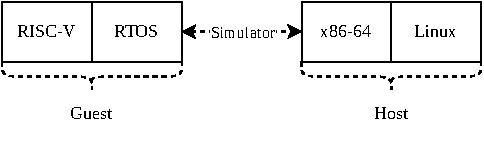
\includegraphics[height=90px]{figures/GuestHostSimulator.pdf}
	\caption{Guest and host with the simulation layer in between}
\end{figure}

% it would be great if you referenced this image in text. Add a \label within the figure, and \ref in text

The machine running the simulator is called the host system, while the simulated system is called the guest or the target
system. The target system instruction set architecture is most often, but not necessarily, different from the host
architecture. The simulator complexity can vary significantly in the domain of complexity and detail.
The extent of the simulation and its verbosity is largely determined by the specific requirements of the application.

According to the Austin et. al \cite{Simplescalar}, three fundamental factors describing the simulator requirements are:

\begin{itemize}
	\item{\textbf{Performance} is the measure of how fast the simulator can finish the specific workload. This metric
	can be described in many ways. One of them being the most intuitive measure of a \textit{relative slowdown/speedup}
	describing the ratio of the time it takes to execute a workload on a simulated hardware, to the time spent
	executing the same workload on the hardware.}
	%
	\item{\textbf{Detail} determines the accuracy of the simulator's state replication in the relation to the hardware,
	which can be described in the terms of how many layers of abstractions are implemented.}
	%
	\item{\textbf{Flexibility} indicates the adaptability of a design. This takes into account factors such as
	portability, modularity, ease of implementing new features, exposed APIs, and many other factors.}
\end{itemize}

It is very difficult to maximize all three of these aspects, and this is the reason why there are so many simulation
solutions available. Most research models tend to optimize performance and flexibility at the expense of detail
\cite{Simplescalar}.

\pagebreak
\section{CPU simulation techniques}

The central processing unit can be simulated in various ways. Each of these simulation methods aims to achieve the same
objective, but employs a distinct approach to the problem. N. Srivastava lists \cite{Nitish-Techniques} these methods:

\begin{itemize}
	\item{\textbf{Functional simulation}, also called an \textbf{Instruction set simulation}, focuses only on the
	fundamental characteristics of the design and correctness of the simulated instruction set architecture,
	% my proposition of slightly changing it.
	i.e. answers the question: "Does this software behave as expected on a given architecture?". Such simulators do not implement any
	timing functionality, and cannot be used to gauge the performance of the simulated architecture. An example of such
	a simulator is Spike, a RISC-V ISA Simulator \cite{Spike}.}
	%
	\item{\textbf{Trace driven simulation}, this type of simulator uses a prerecorded session (\textit{trace}), that is
	later used to simulate the CPU behavior. The trace can be generated either by an existing hardware device or
	using software-based techniques, such as hardware monitoring, binary instrumentation, or trace synthesis
	\cite{Simplescalar}. This method has numerous benefits, such as full determinism, as the whole simulation is
	encapsulated in the trace file. However, since such simulators are limited to simulating traces, they
	cannot easily run arbitrary code. Additional disadvantages of this approach are the requirement for a large
	amount of data storage space, and the poor performance when simulating parallel or timing-dependent systems
	\cite{TraceDrivenAccuracy}. An example of such simulator is gem5 \cite{gem5}, specifically, the \textit{TraceCPU}
	and \textit{Elastic Traces} \cite{gem5trace}.}
	%
	\item{\textbf{Execution driven simulation}, these simulators combine timing and functionality together
	\cite{Nitish-Techniques}, by \textit{executing} the guest instructions, as if they were executed on the hardware.
	This is achieved by translating or interpreting the guest binary code, to the host code (or if the guest
	architecture matches the host's architecture, directly executing the code). Since no traces are needed, the
	% While referencing Hennessy is always a good idea, what do you mean by one machine? As opposed to what?
	simulation can be performed without a trace generator, using only one machine \cite{TraceDrivenAccuracy}.
	The accuracy of the simulation is exclusively determined by the accuracy of the simulator, and the levels of
	abstraction chosen by the simulator developers. Examples of such simulators are the beforementioned QEMU and
	% I assume you also include Renode here? We can't really say "qemu is here, so Renode is automatically covered", Renode is far from being qemu++.
	Dromajo \cite{Dromajo}.}
\end{itemize}

This work will focus solely on the \textbf{execution driven simulators}, but it is important to understand the
different approaches and their purpose. The table \ref{tab:simulators} summarizes this classification:

% frankly i'm not a great fan of this distinction, but naming is not a settled thing, so I won't object
\begin{table}[h]
	\centering
	\begin{tabular}{l|l}
	Type 				& Purpouse 																			 \\ \hline
	Functional 			& \makecell{Validate and verify the correctness of the instruction set architecture} \\ \hline
	Trace 				& \makecell{Simulate the architecture and performance of the processor} 			 \\ \hline
	Execution driven 	& \makecell{Simulate the actions of a processor, rather than the underlying \\
									mechanisms by which it performs those actions}
	\end{tabular}
	\caption{Simulation types}
	% ref needs to go after a caption. Always have them anyway
	\label{tab:simulators}
\end{table}

\pagebreak
\section{Execution driven CPU simulators}

Execution driven simulators can be further divided into two distinct types:

\begin{itemize}
	\item{\textbf{Translation simulators} use dynamic, just-in-time (\textit{JIT}) recompilation of the binary.
	When simulating a CPU architecture that differs from that of the host system,%
	\footnote{If the host and guest architectures match, the translation process can, but does not have to, be skipped,
	by implementing virtualization mechanisms, such as QEMU's KVM \cite{QemuKVM}, or other hypervisor based approaches.}
	% "involves" appears a lot in this paragraph. Not an error, but you might want to reword it a little
	the process of executing guest code involves two phases. The first phase involves interpreting the guest code into
	an intermediate (architecture-independent) representation. The second phase involves recompiling the intermediate
	code into host architecture code, which is subsequently executed on the host's CPU. This process is called
	\textit{Dynamic Binary Translation}, often referred to simply as \textit{translation}.%
	\footnote{While the intermediate code representation is \textit{not} necessary, it allows for a greater degree of
	flexibility and portability.}

	The translated code can be organized into blocks called \textit{Translation Blocks}, which can be cached and
	% this citation is not very specific... I would rather refer to your chapters (with \ref), where you describe both concepts
	chained \cite{Qemu}.

	Such optimizations greatly improve the performance (\textit{redcuce the relative slowdown}), at the
	cost of a complicated simulator codebase. Moreover, this technique implies limited portability, as there is a need
	to implement a new recompiler for each host CPU architecture.

	This method of execution driven simulation will be described thoroughly in Chapter 3, on the example of Renode's
	\textit{Translation library} \cite{Tlib}.}
	%
	\item{\textbf{Interpretation simulators} work by \textit{interpreting} the guest binary. Firstly the simulator
	reads (\textit{fetches}) the opcode, then parses (\textit{executes}) said opcode according to the ISA standards.
	The execution is implemented as a modification of an internal CPU state, which is stored in memory as a data type,
	describing the CPU features and state, such as registers, exception flags, etc.

	% well, it DOES execute code, but not the one it generates
	Since this type of simulator \textbf{does not} does not generate any code for execution on the host's CPU, the recompilation step is not
	necessary. This greatly simplifies the simulator codebase and increases portability. On the other hand, the lack of
	features, such as translation blocks, makes various optimization techniques not possible.

	One example of such a simulator is Dromajo \cite{Dromajo}. The details of its implementation will be described in
	Chapter 4.}
\end{itemize}


\section{Whole-system simulation}

To fully understand the topic of simulation, the reader must also grasp the concept of whole-system simulators. Whole
system simulators implement a beforementioned CPU simulator, alongside peripheral support. Peripherals might be
modeled as a simulation element, or might be passed through to a physical, hardware device. For example, the peripheral
equipment for an embedded system might consist of:
\begin{itemize}
	\item{Serial interfaces,}
	\item{General-purpose input/output,}
	\item{Communication devices, such as I$^2$C, SPI and network controllers.}
\end{itemize}

\pagebreak
\section{Other notable simulators types}

The definition of simulation is broad and extends beyond system emulation. Solutions such as WINE, VMWare Workstation
and QEMU user-mode emulation focus on distinct goals and approaches:

\begin{itemize}
	\item{\textbf{WINE}, recursive backronym for \textit{Wine Is Not an Emulator} \cite{Wine}, is essentially an MS
	Windows API wrapper. This simulator does not attempt to emulate the underlying architecture of the hardware.
	Instead, it focuses on solely simulating software-defined system calls (\textit{syscalls}).}
	%
	\item{\textbf{VMWare Workstation} \cite{VMWareWorkstation} and \textbf{VirtualBox} \cite{VirtualBox}, both of these
	focus on system emulation, but their emulation scope is focused only on simulating an x86 and AMD64/Intel64 machines.
	They operate on the principle of virtualization, to create so-called \textit{virtual machines}. Virtualization
	software directly executes unprivileged code on the host processor. If the host's processor does not support
	x86 virtualization extensions, such as Intel's \textit{VT-x} or AMD's \textit{AMD-V}, the privileged code is firstly
	translated, and then ran on the host. If the host's CPU supports the beforementioned extensions, the guest code does
	not need to be translated.

	Both of mentioned software are referred to as \textit{Level 2 Hypervisors}, as they run on top of the host
	operating system. There are also commercial and open source \textit{Level 1 Hypervisors}, behaving
	as an operating system that is used to provide better guests performance, by the means of providing better and more
	performant access to the underlying hardware \cite{Graniszewski_Waldemar_Performance_2016}.}
	%
	\item{\textbf{QEMU user-mode}, this solution enables the execution of binaries compiled for a different CPU
	architecture on the host system. This approach not only translates the code from the guest to the host but
	additionally translates system calls, handles POSIX signals, and enables proper threading support
	\cite{QemuUser}.

	This solution is useful when creating and debugging Linux and BSD-based applications intended for embedded devices}
\end{itemize}

Unfortunately, these methods of simulation are unsuitable for the creation and testing of embedded devices due to their
restrictive nature and limited capabilities. In particular, their inability to simulate other architectures, limited
% avoid big quantifiers, or you'll have to defend them
debugging capabilities, and lack of customizability for system peripherals make them difficult to be utilized in this
context.

\section{Conclusions}

In this chapter, we briefly examined the existing CPU simulation techniques and their purposes. We divided execution
driven simulators into two distinct types, described the process of the whole system simulation, 
% what do you mean by "and example peripheral in the context of embedded devices"?
and example peripheral
in the context of embedded devices, finally, we finished by mentioning other noteworthy simulators.

Overall, for most cases, the Execution-driven CPU simulator combined with a whole-system emulation framework will be the
most suitable option for most IoT and embedded device development teams, as it provides the needed flexibility, is able
to run arbitrary workloads, and can provide an in-depth look at the guest system.

The hypervisor and syscalls emulators are not functionality rich enough to demonstrate their value in the IoT and
embedded devices development cycle where direct interaction with the hardware layer is an important part of the programmer's work.

\chapter{CPU simulation using translation}

The general concept of the CPU simulation using translation implements the notion of, in a literal sense, translating
code from one instruction set to another, this code is later natively executed on the host CPU. This chapter aims to
provide an overview of the general concept and ideas involved in simulating a central processing unit using translation,
potential optimizations, and challenges in implementing such an approach.

Code snippets from Renode's CPU Translation library (\textit{Tlib})  will be provided to support the explanations, but
all of the described techniques can be also applied to QEMU unless stated otherwise. This document will mainly focus on
the generic and RISC-V specific parts of the code.

\section*{Simulator building blocks}

Understanding the inner workings of such simulators may initially seem intimidating. Therefore, before examining the
individual components, it is important to divide the simulation process into the following phases:

\begin{itemize}
    \item{\textbf{Code translation}, this phase is responsible for parsing the guest binary to the host architecture.
    In our example this is realized by QEMU's \textbf{Tiny Code Generator}.}
    \item{\textbf{Translated code caching}, this process is a key distinguishing factor for translation simulators.
    Since parts of the translated code can be contained in individual entities, they can be cached to increase the speed
    of execution by the means of reducing simulator overhead. In our case, this functionality uses the mechanism of
    \textbf{Translation Blocks}.}
    \item{\textbf{Code execution}, this is the final step for an execution driven simulator. In this section, we will
    examine the various problematic states in which the simulator can find itself. This covers the things such as
    I/O access, MMU, etc.}
\end{itemize}

\section{Code translation}

Translation CPU simulation (later referred to as \textit{Translators}), as the name implies, relies on the ability to
translate the code from one architecture, to another. The translation step might be accompanied by a translation to an
intermediate representation. Such is the case in our example with the Tiny Code Generator (later referred to as
\textit{TCG}), where the guest code is at first translated to an intermediate, architecture independent representation,
to be later translated into the host code.

\pagebreak

% image here showing the TCG layers
\begin{figure}[h]
	\centering
	\vspace{10px}
	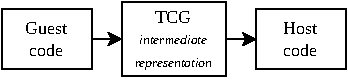
\includegraphics[height=70px]{figures/Translation_Guest-TCG-Host.pdf}
	\caption{TCG translation process}
\end{figure}

\noindent
The translation process is twofold, first phase consists of translating the guest code, for example a RISC-V compiled
workload, to an \textbf{TCG Intermediate Representation} (referred to as \textit{TCG IR}), this part is
called \textit{The frontend}. The second phase translates the TCG IR to the host ISA code, this part is called
\textit{The backend}.%
\footnote{Such notion of the backend and frontend operations allows the simulator to separate the adaptation
of new guest and host architectures, making the simulator more flexible.}

The following sections will only explain the basics of both TCG operations, as these mechanisms are very
complicated. Note that this flow only happens when there is no cached Translation Block found. The topic of TBs and
their caching will be explained later, for now, we only care about the code translation mechanisms.

\subsection{Main execution loop}

The main CPU execution method, \texttt{cpu\_exec()}, tries to find a cached translation block using
\texttt{tb\_find\_fast()}, if this fails the \texttt{tb\_find\_slow()} is called. If a block is found, the host starts
executing the translated code. If this function does not find the block, the \texttt{tb\_gen\_code()} is called.
This function allocates memory for a to-be-created translation block and sets needed flags in it. After that is done,
the \texttt{cpu\_gen\_code()} is called:

\nopagebreak[4]
\begin{lstlisting}[
    style=lstC,
    label={lst:cpu-gen-code},
    caption={The \texttt{cpu\_gen\_code()} code. Variable declaration omitted.}
    ]
void cpu_gen_code(CPUState *env, TranslationBlock *tb, ...)
{
    tcg_func_start(s);
    cpu_gen_code_inner(env, tb);

    /* generate machine code */
    gen_code_buf = tb->tc_ptr;
    tb->tb_next_offset[0] = 0xffff;   tb->tb_next_offset[1] = 0xffff;

    s->tb_next_offset = tb->tb_next_offset;
    s->tb_jmp_offset = tb->tb_jmp_offset;
    s->tb_next = NULL;

    gen_code_size = tcg_gen_code(s, gen_code_buf);
    *gen_code_size_ptr = gen_code_size;

    search_size = encode_search(tb, gen_code_buf + gen_code_size);
    *search_size_ptr = search_size;
}
\end{lstlisting}

\subsection{TCG frontend}
\label{sec:tcg-frontend}

The first two calls from the code (\ref{lst:cpu-gen-code}), are responsible for generating an intermediate
representation. The \texttt{tcg\_func\_start()} initializes TCG, while the \texttt{cpu\_gen\_code\_inner()} prepares
\textit{DisasContext},%
\footnote{A DisasContext typically includes information such as the address of the machine code being disassembled,
the size of the code, and the type of CPU architecture the code is intended for. It may also include pointers to other
data structures or functions that are used by the disassembler}
and starts a translation loop.

The main part of the translation loop is the \texttt{gen\_intermediate\_code()} call, this is a platform-specific
IR generation method. This function later calls the \texttt{disas\_insn()} routine, responsible for disassembling
the instruction, I.e. in the RISC-V implementation this function determines whether the type of opcode under the current
program counter (is it a compressed instruction? does the opcode belong to a custom extension?). After determining
the type of the opcode, the according decode function is called. Since we are considering RISC-V ISA, the decode function
is \texttt{decode\_RV32\_64G()}. The decode function then parses opcode according to the ISA standard, and calls a
function that will generate IR opcodes:

\begin{lstlisting}[
    style=lstC,
    label={lst:decode-rv32},
    caption={Opcode decoding on an example of RISC-V \texttt{addi}.}
    ]
static void decode_RV32_64G(CPUState *env, DisasContext *dc)
{
    op = MASK_OP_MAJOR(dc->opcode);
    rs1 = GET_RS1(dc->opcode);
    rs2 = GET_RS2(dc->opcode);
    rd = GET_RD(dc->opcode);
    imm = GET_IMM(dc->opcode);
    rm = GET_RM(dc->opcode);

    switch (op) {
        case OPC_RISC_ARITH_IMM:
        gen_arith_imm(dc, MASK_OP_ARITH_IMM(dc->opcode), rd, rs1, imm);
        break;
        ...
    }
}

static void gen_arith_imm(DisasContext *dc, uint32_t opc, int rd, int rs1, long imm)
{
    switch (opc) {
    case OPC_RISC_ADDI:
        tcg_gen_addi_tl(source1, source1, imm); //#define tcg_gen_addi_tl   tcg_gen_addi_i32
        break;
    ...
    }
}
\end{lstlisting}

\noindent
The translation loop continues indefinitely until one of the following conditions is met:
\begin{itemize}
    \item{Number of instructions in TB has reached a maximum allowed value, or an error occurred,}
    \item{There are breakpoints defined, and the breakpoint address matches the current PC,}
    \item{Last translated opcode is a jump instruction.}
\end{itemize}

\pagebreak
\subsection{TCG backend}

The rest of the function from (\ref{lst:cpu-gen-code}) is responsible for recompiling an IR to the host architecture.
The first part of the code prepares the translation block and can be skipped for now. The actual transition occurs
in the \texttt{tcg\_gen\_code()} function:

\begin{lstlisting}[
    style=lstC,
    label={lst:tcg-gen-code},
    caption={IR to host encoding.}
    ]
static inline int tcg_gen_code_common(TCGContext *s, uint8_t *gen_code_buf)
{
    for (;;) {
        opc = tcg->gen_opc_buf[op_index];
        def = &tcg_op_defs[opc];
        switch (opc) {
        case INDEX_op_movi_i32:
            tcg_reg_alloc_movi(s, args);
            break;
        ...
        case INDEX_op_call:
            dead_args = s->op_dead_args[op_index];
            args += tcg_reg_alloc_call(s, def, opc, args, dead_args);
            goto next;
        case INDEX_op_end:
            goto the_end;
        ...
        default:
            dead_args = s->op_dead_args[op_index];
            tcg_reg_alloc_op(s, def, opc, args, dead_args);
            break;
        }
    }
}
\end{lstlisting}

\noindent
This method handles special IR micro-ops first, such as exiting the block or calling a helper function (more about them
later). If the \texttt{opc} does not match any of the special cases, the code falls through to the \texttt{default}
block, where the \texttt{tcg\_reg\_alloc\_op()} is called, witch then calls target-specific \texttt{tcg\_out\_op()} method.

\begin{lstlisting}[
    style=lstC,
    label={lst:tcg-out-op},
    caption={Generating \textit{target} instructions from IR.}
    ]
static inline void tcg_out_op(TCGContext *s, TCGOpcode opc, const TCGArg *args, ...)
{
    switch(opc) {
        case INDEX_op_exit_tb:
            tcg_out_movi(s, TCG_TYPE_PTR, TCG_REG_EAX, args[0]);
            tcg_out_jmp(s, (tcg_target_long) tb_ret_addr);
            break;
        case INDEX_op_br:
            tcg_out_jxx(s, JCC_JMP, args[0], 0);
            break;
    }
}
\end{lstlisting}

\pagebreak
\subsection{Example of code translation using TCG}

The best way to illustrate the operations of TCG, is to provide an example, let's look at an example of RISC-V to IR to
x86 translation. This example comes from booting a Zephyr RTOS "Hello World" demo on a QEMU-RV32 system:%
\footnote{The QEMU flags to create such logs: \texttt{-d in\_asm, -d out\_asm, -d op}.}

\begin{itemize}
    \item{RISC-V guest machine code:
    \begin{lstlisting}[frame=tblr]
    0x00001000:  00000297          auipc           t0,0            # 0x1000
    0x00001004:  02828613          addi            a2,t0,40
    0x00001008:  f1402573          csrrs           a0,mhartid,zero
    \end{lstlisting}
    }
    %
    \item{TCG IR micro-ops:
    \begin{lstlisting}[frame=tblr, label={lst:tcg:tcgir-microops}]
    0x00001000:   mov_i32 x5/t0,$0x1000
    0x00001004:   add_i32 x12/a2,x5/t0,$0x28
    0x00001008:   mov_i32 tmp5,$0x1
                  st_i32 tmp5,env,$0xfffffffffffff1a8
                  call csrr,$0x0,$1,x10/a0,env,$0xf14
                  mov_i32 pc,$0x100c
                  exit_tb $0x0
                  set_label $L0
                  exit_tb $0x7fef28000043
    \end{lstlisting}
    }
    %
    \item{x86 host machine code:%
    \footnote{The \texttt{callq} opcode uses \textit{RIP Relative Adressing}, allowing the call location to be
    intermixed with the code. Using GDB it was possible to verify that \texttt{0x000055a84d2b8e00}
    was the addres of an according helper function.}
    \begin{lstlisting}[frame=tblr, label={lst:tcg:x86translated}]
    0x7eff7c000123:  c7 45 14 00 10 00 00           movl     $0x1000, 0x14(%rbp)
        -- guest addr 0x00001004
    0x7eff7c00012a:  c7 45 30 28 10 00 00           movl     $0x1028, 0x30(%rbp)
        -- guest addr 0x00001008
    0x7eff7c000131:  c7 85 a8 f1 ff ff 01 00        movl     $1, -0xe58(%rbp)
    0x7eff7c000139:  00 00
    0x7eff7c00013b:  48 8b fd                       movq     %rbp, %rdi
    0x7eff7c00013e:  be 14 0f 00 00                 movl     $0xf14, %esi
    0x7eff7c000143:  ff 15 1f 00 00 00              callq    *0x1f(%rip)
    0x7eff7c000149:  89 45 28                       movl     %eax, 0x28(%rbp)
    0x7eff7c00014c:  c7 85 18 12 00 00 0c 10        movl     $0x100c, 0x1218(%rbp)
    0x7eff7c000154:  00 00
    0x7eff7c000156:  e9 bb fe ff ff                 jmp      0x7eff7c000016
    0x7eff7c00015b:  48 8d 05 e1 fe ff ff           leaq     -0x11f(%rip), %rax
    0x7eff7c000162:  e9 b1 fe ff ff                 jmp      0x7eff7c000018
    ...
    data: [size=8]
    0x7eff7c000168:  .quad  0x000055a84d2b8e00
    \end{lstlisting}
    }
\end{itemize}

\noindent
The \textit{TB Prologues} have been omitted, as they will be covered in a section discussing the translation blocks.
Upon further inspection, one can notice that the guest \texttt{csrrs} opcode has emitted an host \texttt{call} opcode.
This brings us to the topic of helper functions.

\pagebreak
\subsection{Helper functions}

Helper functions serve the purpose of emulating incompatible instructions by delegating their execution to the
simulation layer, essentially bypassing the main TCG translation mechanisms. Examples of such functions include
architecture-specific instructions, for example, accessing guests' control and status registers, and memory access
instructions, which are handled by SoftMMU.

Helper functions are akin to the idea of callbacks or trampolines in higher-level programming languages. Helpers calls
are dynamically included in the TCG IR, when the opcode gets parsed in the decode function (for example in previously
mentioned (\ref{lst:decode-rv32})).

These are not called directly in code, both Tlibs and QEMU implement helper generation evil pre-processor macros.


\begin{lstlisting}[
    style=lstC,
    label={lst:csrrs-helper},
    caption={RISC-V \texttt{csrrs} helper.}
    ]
target_ulong helper_csrrs(CPUState *env, target_ulong src, target_ulong csr, target_ulong rs1_pass)
{
    validate_csr(env, csr, rs1_pass != 0);
    uint64_t csr_backup = csr_read_helper(env, csr);
    if (rs1_pass != 0) {
        csr_write_helper(env, src | csr_backup, csr);
    }
    return csr_backup;
}
\end{lstlisting}

\section{Translation Blocks}

The previously described translation process may seem overly convoluted, but when paired with the ability to cache and
reuse translated code, it significantly enhances the overall performance of the simulator. This is immensely important
in this context, as speed is one of the main distinguishing features of QEMU and Tlib.

Building up upon the knowledge from the previous section, when TCG is translating the code, it divides the
code into the \textbf{smallest possible standalone pieces of code}, by this, we understand the code that has only one
possible exit point. In other words, translation blocks always end on:
\begin{itemize}
    \item{Branching instructions, including both conditional and unconditional jumps, calls, and returns.}
    \item{Helper callbacks, because they call an external code, the TB execution must be halted. This can be seen
    in the TCG IR micro-ops (\ref{lst:tcg:tcgir-microops}) example, where the \texttt{tb\_exit} micro-op is emitted
    after an \texttt{csrrs} helper was called.}
\end{itemize}

In the case of conditional branches, the QEMU and Tlibs implement a \textit{Lazy evaluation of the CPU condition codes},
as in, the TCG only translates one path of the branching instruction. If the TCG were to generate native machine code
for both the taken and not-taken paths of the branch, it would have to generate twice as much machine code as is needed.
By using lazy evaluation, the TCG can generate the native machine code for the taken path of the branch only when the
branch is taken, rather than generating machine code for both paths in advance \cite{QemuInternalsTech}.

\pagebreak
\begin{figure}[h]
	\centering
	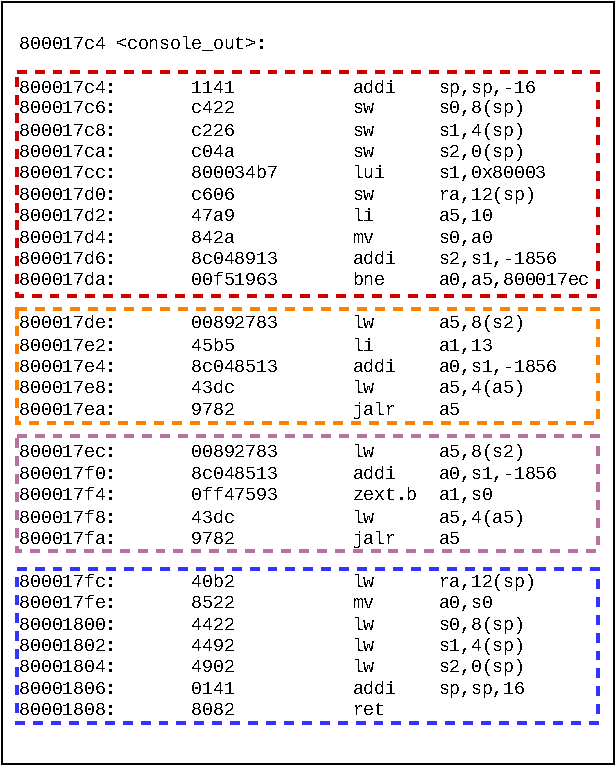
\includegraphics[height=400px]{figures/TranslactionBlocks.pdf}
	\caption{An example of basic block division.}
    \label{fig:block-division}
\end{figure}

\subsection{Translation Block caching}

After each block translation, the translated block is appended to the \textbf{TCG Translation Block Cache}.
The QEMU Internals, states that "A 32 MByte cache holds the most recently used translations. For simplicity, it is
completely flushed when it is full" \cite{QemuInternalsTech}. The cache also needs to be flushed when the code modifies
itself, this is accomplished by setting a host memory page holding the code to be read-only. Then if the
write-protected region is modified, the Linux will emit a \texttt{SEGV} signal, that will be handled by QEMU. This
invalidates and flushes the cache, as well as flushes direct block chaining lists.

This feature significantly improves the performance of the simulator, as the code usually needs to be translated only
once, significantly reducing the simulation overhead. This optimization also enables another performance improvement,
that aims to mitigate the performance penalty needed for the context switch between the translated guest code and the
QEMU runtime. This will be described in the next section.

\pagebreak
\subsection[Translation Block chaining]{Translation Block chaining
\footnote{A notable portion of the images in this section was inspired by Chad D. Kersey's presentation
\cite{QemuInternalsPresentation}.}}

Block chaining is a technique used to reduce the time spent on context switching between translated guest code and the
runtime of the simulator. The majority of the context switch time comes from the fact that the CPU state, such as
registers and status flags, has to be saved into memory. Memory operations and context swaps tend to be
the slowest things a CPU does, as they might require up to a hundred cycles.
% mabye put some google scheduler slides idk?

\subsection*{No block chaining}

Assuming there is no block chaining, each block execution will look like this:
\begin{figure}[h]
	\centering
	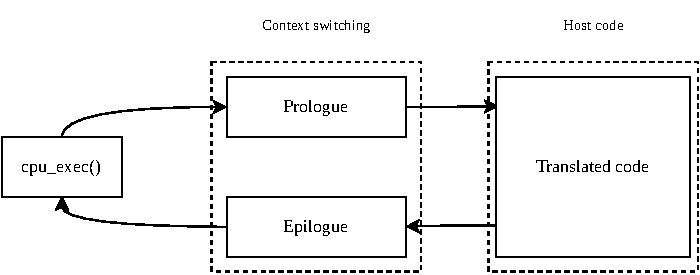
\includegraphics[width=0.75\textwidth]{figures/TbExecution-NoChain.pdf}
	\caption{Execution flow with no block chaining}
\end{figure}

\noindent
The \textit{Context switching} block consists of two elements, a \textit{Prologue} and an \textit{Epilogue}. The former
saves the Runtime context, swaps the previously saved context to the host code execution, and jumps to the code pointer.
The latter saves the host code execution context, restores the simulator runtime context, and jumps to the
\texttt{cpu\_exec()} loop.
Looking at the example Translation Blocks from Fig. (\ref{fig:block-division}), one might notice that returning to a
main loop after each block execution will cause a lot of context switching, which would be a huge detriment to the
overall performance of the simulator.

\subsection*{Direct block chaining}

To mitigate this issue, the QEMU developers came up with a mechanism, that chains the block execution. This allows the
simulator to directly link each block with another, greatly reducing the overhead from context swapping.
This comes at the price of increased code complexity and additional possible issues stemming from the
self-modifying code, with the latter being especially prevalent in the SMP system emulation.

This is accomplished by leaving extra space in a translated code, just before a return to the epilogue. Later, when
the code is finished executing and has not been patched to jump to any other TB, the block returns to the epilogue,
in turn, exits to the \texttt{cpu\_exec()}. The main loop then tries to chain this block, to the next block. This
process is repeated for every exiting block.

There are other ways to chain TB that do not require exiting the host code, instead, these methods are executed at the
translation phase of the code. These mechanisms are explained in detail in the QEMU Translator Internals documentation,
at the Direct block chaining section \cite{QemuDocsChaining}.

\pagebreak

\begin{figure}[h]
	\centering
    \label{fig:qemu-execution-with-blocks}
	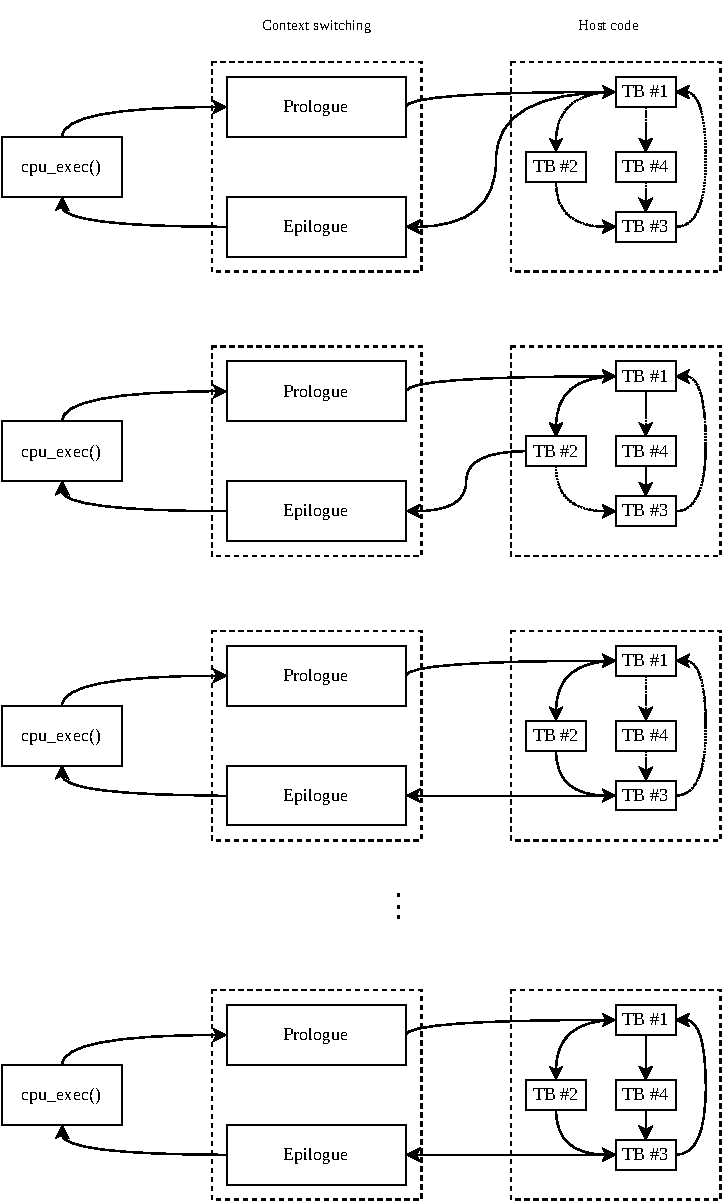
\includegraphics[width=0.7\textwidth]{figures/TbExecution-Chain.pdf}
	\caption{Execution flow with block chaining}
\end{figure}

\noindent
This relatively simple mechanism can create high-speed execution loops, even to the point where the host code
might not exit a loop for a very long time.

This is an interesting case, because such behavior can be classified as
blocking, and might be an issue when dealing with asynchronous interrupts. Let's assume that the binary doesn't fill up
the whole transition cache, the code never overwrites itself, and the TBs have been patched in a way that creates a
loop. In such cases, handling asynchronous exceptions is not possible, as the code never exits back to the main loop.

This problem has been solved by adding another thread, that is polling for interrupts, and if one is received, the
simulator will invalidate all of the TB's chains, exiting to the main loop at the end of the current TB.

\pagebreak

\section{Code Execution}

In the final section of this chapter, we will examine various issues and questions that may arise during the execution
of translated code.

\subsection{Staring the execution of the translated code}

When the simulator finds the Translation Block it executes the \texttt{tcg\_tb\_exec()} function, which is a
macro-definition, which casts a translation buffer to a function pointer, then calls it with arguments.

\begin{lstlisting}[
    style=lstC,
    caption={Executing the translation buffer.}
    ]
int cpu_exec(CPUState *env)
{
    ...
    env->current_tb = tb;
    asm volatile ("" ::: "memory");
    if (likely(!env->exit_request)) {
        tc_ptr = tb->tc_ptr;
        /* execute the generated code */
        next_tb = tcg_tb_exec(env, tc_ptr);
    }
    ...
}

#if !defined(tcg_tb_exec)
#define tcg_tb_exec(env, tb_ptr) \
    ((uintptr_t REGPARM (*)(void *, void *))tcg->code_gen_prologue)(env, tb_ptr)
#endif
\end{lstlisting}

\subsection{Exception and interrupt handling}

Exceptions and interrupts are an inseparable part of the CPU simulation, without them, the CPU would not be able to
handle most workloads. The logic handling them is fully architecture dependent, but this section will cover the
generic code. All of the examples are shown using a RISC-V instruction set.

By exception, we understand an event that occurs from the CPU itself. These events might happen upon user request, such
as \texttt{ecall} instruction or they might happen spontaneously, for example, a \texttt{mbadaddr} condition.

The term interrupts, often referred to as asynchronous exceptions, are a result of an external device sending an
interrupt request (\textit{IRQ}) to the CPU. An example of such an event is an External Timer sending an interrupt that
compares time has been reached, or a network device to signal that a new packet is ready to be handled.

\pagebreak
\subsection*{Exception generating}
The exceptions are generated using the beforementioned helper functions:

\begin{lstlisting}[
    style=lstC,
    caption={Generating exceptions using handlers.}
    ]
static inline void __attribute__ ((__noreturn__))
do_raise_exception_err(CPUState *env, uint32_t excpt, uintptr_t pc, uint32_t call_hook)
{
    env->exception_index = excpt;
    cpu_loop_exit_restore(env, pc, call_hook);
}

...

void helper_raise_exception_mbadaddr(CPUState *env, uint32_t excpt, target_ulong bad_pc)
{
    env->badaddr = bad_pc;
    do_raise_exception_err(env, excpt, 0, 1);
}
\end{lstlisting}

\subsection*{Interrupt generating}
The interrupts are generated in a different flow. A virtual device can \textit{send} an interrupt, by setting the
\texttt{exception\_index} to a value matching the ISA standards. The rest of the flow is identical to the exception
handling.

In the case of the QEMU, the interrupts are handled by the QEMU system module. In Renode's Tlibs, the external
interrupts are sent from the Renode framework, in this scenario extra care needs to be put in when dealing with
interrupt requests, such as using atomic operations, using locks on variables, etc.

\subsection*{Handling the exceptions in the main loop}

The main loop makes use of C library \texttt{setjmp/longjmp} for exception handling inside the simulated CPU.
The \texttt{setjmp} env is set just before the main execution loop. If the exception occurs the execution loop handles
the exception, then using \texttt{longjmp} jumps back to the point before an event occurred. This implementation allows
the CPU thread to exit deep and complex TCG translation functions.

It is worth noting that exceptions and interrupts are handled by the same function, the only aspect where they are
different is a way, in which the event is generated.

\pagebreak

\begin{lstlisting}[
    style=lstC,
    caption={Handling exceptions in the main loop.}
    ]
int cpu_exec(CPUState *env)
{
    env->exception_index = -1;
    /* before TB execution */
    for (;;) {
        if (setjmp(env->jmp_env) == 0) {
            if (env->exception_index >= EXCP_INTERRUPT) {
                ret = env->exception_index;
                // An event is an exception, not an interrupt
                // Skip to the second for loop, and handle it there
                break;
            } else {
                do_interrupt(env);
            }
        }
        ...
        /* TC execution */
        for(;;)
        {
            if (unlikely(env->exception_index != -1)) {
                cpu_loop_exit_without_hook(env);
            }
        }
    ...
\end{lstlisting}

\noindent
The events are then handled in the architecture specific \texttt{do\_interrupt()} function:

\begin{lstlisting}[
    style=lstC,
    caption={Generating interrupts using \texttt{do\_interrupt()}.}
    ]
void do_interrupt(CPUState *env)
{
    if (env->nmi_pending > NMI_NONE) {
        do_nmi(env);
        return;
    }
    if (env->exception_index == EXCP_NONE) {
        return;
    }
    ...
    if (env->priv == PRV_M || !((is_interrupt ? env->mideleg : env->medeleg) & (1 << bit))) {
    /* handle the trap in M-mode */
    env->mepc = env->pc;
    env->mcause = fixed_cause;
    if (hasbadaddr) {
        env->mtval = env->badaddr;
    }
    ...
}
\end{lstlisting}


\chapter{CPU simulation using interpretation}

CPU simulators using interpretation are more akin to functional simulators, as they directly implement
functional characteristics in the simulator code, without any translation layers. This chapter aims to provide a
general overview of the mechanisms used in such simulators and compare the general concepts with translation
simulators.
% I would skip this sentence tbh
Because of their inherent simplicity, this chapter will be much shorter than the previous one.

Code snippets from the Dromajo RISC-V CPU simulator will be provided to support the explanations. This document will not
cover Dromajo's implementation of machine simulation, but will focus mainly on the CPU simulation aspect.

\section*{Interpretation simulator fundamentals}

Since the code doesn't need to be translated, the simulator directly executes the loaded binary. As is the case with
QEMU and Renode Tlib's, Dromajo also implements a virtual memory management unit, although this implementation is
simplified, implementing only \texttt{sv39} and \texttt{sv48} page based virtual-memory systems \cite{RISC-PRIV}. % as compared to... ?

After the code has been loaded and the program counter has been set to the correct value, the interpretation method
can be called. In the case of the Dromajo, the method starting the execution is \texttt{riscv\_cpu\_interp()}, which
then calls either \texttt{riscv\_cpu\_interp32} or \texttt{riscv\_cpu\_interp64()}, defined in the \texttt{dromajo\_template.h} file. The simulator then
enters the main execution loop, which checks for interrupts, TLB status, and finally proceeds with the interpretation of the code.

\section{Code interpretation}

The code interpretation is a step equivalent to the TCG Frontend, described in the section \ref{sec:tcg-frontend}.
The loaded instruction is separated into an opcode and operands. After that, the simulator interprets the instruction
and executes it by modifying the internal CPU state.

Lack of a translation process is a key characteristic that distinguishes interpretation CPU simulators from their
translation counterparts, and is one of the main arguments in favor of using interpretation simulators, as they
% I don't understand "They do not require guest to host or intermediate representation"
are inherently portable. They do not require guest to host or intermediate representation to host translators, which
means that they can be used with any architecture they can be compiled for.

Since Dromajo is written in pure \texttt{C++} and uses \texttt{CMake} as the build system, it can be run on most, if not all,
% Wait, whaaaaat? All operating systems? You mean Linux/Windows/macOS only? :> Also, cmake does not really improve portability imho. Portability across archs is guaranteed when you don't use asm and don't use libs that are not portable 
of the current operating systems and architectures.

\pagebreak

\section{Code execution}

Code execution takes place in the main execution loop, a concept similar to the QEMU main execution loop.

\begin{lstlisting}[
    style=lstC,
    label={lst:dromajo-interpret},
    caption={The Dromajo instruction interpretation.}
    ]
int no_inline glue(riscv_cpu_interp, XLEN)(RISCVCPUState *s, int n_cycles) {
    for (;;) {
    ...
    opcode = insn & 0x7f;
    rd     = (insn >> 7) & 0x1f;
    rs1    = (insn >> 15) & 0x1f;
    rs2    = (insn >> 20) & 0x1f;
    switch (opcode) {
        ...
        case 0x37: /* lui */
                if (rd != 0)
                    write_reg(rd, (int32_t)(insn & 0xfffff000));
                NEXT_INSN;
        case 0x17: /* auipc */
            if (rd != 0)
                write_reg(rd, (intx_t)(GET_PC() + (int32_t)(insn & 0xfffff000)));
            NEXT_INSN;
        ...
    }
\end{lstlisting}

\noindent
This \texttt{switch/case} block contains all of the supported instructions. After executing the instruction, the code
executes the \texttt{NEXT\_INSN} macro, which expands to \texttt{code\_ptr += 4; break}, incrementing the code pointer,
exiting the switch block, and returning to the beginning of the main loop. This process is then repeated indefinitely,
until an exception or an interrupt is raised, or the simulator finishes executing the requested amount of
instructions.

\section{Exception and interrupt handling}

Similar to the case of QEMU and Tlib, both exceptions and interrupts are handled by the same function, with the only
the difference being the way they are generated.

\subsection*{Exception generation}

An exception can be triggered for example upon execution of a trap raising instruction, such as \texttt{ecall}:

\begin{lstlisting}[
    style=lstC,
    label={lst:dromajo-generate-exception},
    caption={Generating an exception in Dromajo.}
    ]
case 0x000: /* ecall */
    if (insn & 0x000fff80)
        goto illegal_insn;
    s->pending_exception = CAUSE_USER_ECALL + s->priv;
    s->pending_tval      = 0;
    goto exception;
\end{lstlisting}

\pagebreak

\noindent
The \texttt{illegal\_insn} and \texttt{exception} labels are found after the end of the main execution loop:

\begin{lstlisting}[
    style=lstC,
    label={lst:dromajo-enter-exception},
    caption={Entering the exception handler in Dromajo.}
    ]
illegal_insn:
    s->pending_exception = CAUSE_ILLEGAL_INSTRUCTION;
    s->pending_tval      = 0;
mmu_exception:
exception:
    ...
    raise_exception2(s, s->pending_exception, s->pending_tval);
\end{lstlisting}

\subsection*{Interrupt generation}

Interrupts requests are checked and generated at the very top of the execution loop:

\begin{lstlisting}[
    style=lstC,
    label={lst:dromajo-generate-interrupt},
    caption={Generating an interrupt in Dromajo.}
    ]
...
/* check pending interrupts */
if (unlikely(((s->mip & s->mie) != 0) && ...)) {
    if (raise_interrupt(s)) {
        goto the_end;
    }
}
...

static int __must_use_result raise_interrupt(RISCVCPUState *s) {
    mask = get_pending_irq_mask(s);

    raise_exception(s, irq_num | CAUSE_INTERRUPT);
    return -1;
}

static inline uint32_t get_pending_irq_mask(RISCVCPUState *s) {
    pending_ints = s->mip & s->mie;
    /* Determine what IRQ's are enabled */
    ...
    return pending_ints & enabled_ints;
}
\end{lstlisting}

\noindent
At the end of the \texttt{raise\_interrupt()} function is called, invoking the same flow as for the exception.

\section*{Handling the exceptions}

Exception and interrupt handling is done in the \texttt{raise\_interrupt()} function, which is an implementation of
a RISC-V exception handling model. This method determines if the event is an IRQ or an internal CPU trap, handles
delegating the event to the lower privilege modes, etc.

\pagebreak

\section{Interpretation CPU simulator flow}

The flow will be presented based on the Dromajo simulator, but it is generally a common approach.

% image here showing the TCG layers
\begin{figure}[h]
	\centering
	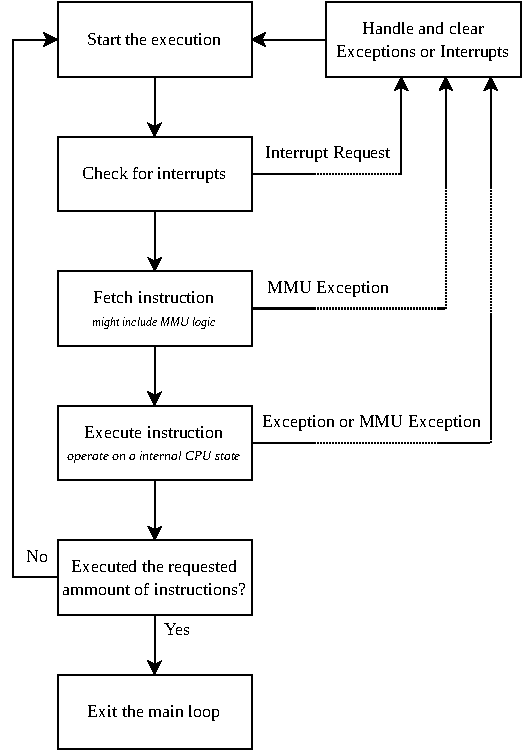
\includegraphics[width=0.75\textwidth]{figures/DromajoFlow.pdf}
	\caption{Interpretation CPU flow}
\end{figure}

\noindent
The flow is much simpler than the one QEMU implements, described in the previous chapter. Keeping in mind the general
simulator constraints mentioned in the second chapter, it should be clear that such simplicity comes at the cost of
performance. An analysis of how much performance is lost due to the lack of optimizations that translation CPU simulators
implement is the main point of this work and will be conducted in Chapter 6.
% I think it's actually chapter 6, right?

\chapter{Integrating Dromajo with Renode framework}

This chapter aims to introduce the reader to general implementation concepts of the integration of the Dromajo simulator with the Renode Framework.
To provide a reader with a better understanding of the integration process, this chapter also covers
the basics of Dromajo and Renode, the structure of simulated devices, and the basics of CPU simulation
implementation in the framework.

In order to integrate Dromajo with the Renode simulation framework, the following steps must be completed:
\begin{itemize}
    \item{creating an external simulator API for Dromajo,}
    \item{creating a DromajoCPU interface in Renode,}
    \item{binding Dromajo's C library to Renode C\# managed code.}
\end{itemize}

\noindent
The process of implementation is outlined in two distinct stages. The first part describes the implementation of an
external simulator API in Dromajo. The second part focuses on the Renode side and covers the details of creating a
DromajoCPU instance and binding C\# managed code to C++ library.

\section{Dromajo}

Dromajo is an Esperanto Technologies RISC-V (RV64GC) emulator designed for RTL co-simulation.%
\footnote{RTL (register-transfer level) co-simulation is a technique used in hardware design and verification to
simulate the behavior of a digital circuit design (CPU) at the RTL level.}
%Hey, this sentence is a copy-paste. NO GO
Dromajo's semantic model is based on Fabrice Bellard's RISCVEMU (later renamed TinyEMU), but extensively verified,
bug-fixed, and enhanced to take it to ISA 2.3/priv 1.11 \cite{Dromajo}.
\footnote{Fabrice Bellard is also the original author of TCG and QEMU.}
It has been released under Chips Alliance
\cite{ChipsAlliance} under an Apache 2.0 License.

Dromajo at the core is either an RTL co-simulation engine or a whole machine emulator, both implementing an
% ideally you'd not write Chapter 4, but Chapter \ref{chap:interpret}. But I'm being picky.
Interpretation CPU emulator, which inner workings have been described in the Chapter 4. Dromajo does not provide any API
% My wording here, about intro work, is deliberate. You remember our discussion about the thesis being about research, not implementation
for integration with other simulators, which was resolved as a part of the introductory work to this thesis. The majority of the
codebase is written in C, but due to a few C++ dependent functionality (for example \texttt{LiveCache}), the project is
compiled as a C++ project, using \texttt{Cmake} build engine.
% Please let me know what is this livecache

%it's usually a bad idea to have manual pagebreaks...
\pagebreak

\subsection{External Simulator API for Dromajo}

The Dromajo CPU simulator operates on an internal emulator state (\texttt{struct RISCVCPUState}), therefore each
instance of the library must implement its own, global-scoped \texttt{*env} state. Since this approach is not considered
% I do not understand. Whose approach was this? Did we enforce global env, did we need it? I don't get it.
a good practice in most cases, the existing methods were not compatible with such approach. This was solved by
creating \texttt{wrappers} for already existing methods, that passed the global state as a parameter to existing
functions. To implement this approach with as few changes to an already existing source code as possible, there was a need to
extract the essential functionality to an independent compile unit.%
\footnote{A compilation unit, often referred to as translation unit, is a final representation of the source code,
from which the object file is generated.}

\vspace{10px}
\noindent
List of exposed API functions (the \texttt{dromajo\_} prefix has been omitted in all function names):
\begin{multicols}{2}
    \begin{itemize}
        \item{\textbf{init\_cpu}\\Initializes the \texttt{*env} state, sets a \texttt{hartid} }
        \item{\textbf{map\_range}\\Registers a RAM page in the emulator}
        \item{\textbf{virt\_to\_phys}\\Translates guest to host RAM address}
        %is this supposed to be bit_bit? I don't think so
        \item{\textbf{set\_mip\_bit\_bit\_state}\\Sets or resets selected MIP CSR flag}
        \item{\textbf{execute}\\Interprets a given number of instructions} % I added "given", becuse it looked like "interprets what the number means"
        \item{\textbf{get\_power\_down\_flag}\\Returns the CPU power down flag}
        \item{\textbf{get\_pc}\\Returns the current program counter}
        \item{\textbf{set\_pc}\\Sets the program counter to a requested value}
        \item{\textbf{get\_hart\_id}\\Returns the CPU \texttt{hartid}}
        \item{\textbf{set\_hart\_id}\\Sets the \texttt{hartid} to a requested value}
        \item{\textbf{get\_register}\\Returns a selected CPU register}
        \item{\textbf{set\_register}\\Sets a CPU register to a requested value}
    \end{itemize}
\end{multicols}

\noindent
The listing below presents a sample implementation:

% wait, is it ACTUALLY bit_bit? That's fishy
\begin{lstlisting}[
    style=lstC,
    label={lst:dromajo-api-state},
    caption={Examples of External Simulator API function wrapper.}
    ]
RISCVCPUState *env;

void dromajo_set_mip_bit_bit_state(uint32_t number, BOOL value) {
    uint32_t mask = 1 << number;

    //The riscv_cpu_* functions are a part of existing Dromajo code
    value ? riscv_cpu_set_mip(env, mask) : riscv_cpu_reset_mip(env, mask);
}

uint32_t dromajo_get_power_down_flag() {
    return riscv_cpu_get_power_down(env);
}
...
\end{lstlisting}

\noindent
This interface is good enough for basic usage, but it does not enable the external simulator to control the CPU
execution flow precisely. This issue is discussed on in the next section.

% pagebreaks are fishy
\pagebreak

% either interface, or api
\subsection{External Simulator API for Dromajo}

To further extend the functionality of the API, the \textit{External Simulator Interface} has been also added
to more comprehensively integrate the CPU emulator into an external simulator. The main motivation for this
feature is the ability to add breakpoints and to provide an organized interface to add callbacks to an external
simulator. This functionality implements a \texttt{struct ExternalSimulator} embedded, as a member, into the
\texttt{RISCVCPUState}.

% duuuuuuude!
\vspace{10px}
\noindent
List of exposed interface API functions (the \texttt{external\_sim\_} prefix has been omitted in all function names):
\begin{multicols}{2}
    \begin{itemize}
        \item{\textbf{init}\\Initializes \texttt{ExternalSimulator} with provided external simulator callbacks}
        \item{\textbf{get\_execution\_stopped\_flag}\\Returns the exit status of the execution:
        \texttt{\{OK,Breakpoint,WFI\}}}
        \item{\textbf{get\_executed\_instructions}\\Returns the ammount of executed insn. since the last call}
        \item{\textbf{check\_breakpoint}\\Checks if breakpoint exists at current PC}
        \item{\textbf{set\_ignore\_bp\_flag}\\Tells the emulator to ignore the next breakpoint}
        \item{\textbf{set\_any\_bp\_flag}\\Tells the emulator to ignore every breakpoint}
        \item{\textbf{add\_breakpoint}\\Adds a breakpoint at a given PC}
        \item{\textbf{remove\_breakpoint}\\Removes a breakpoint at a given PC}
    \end{itemize}
\end{multicols}

\noindent
The listing below presents a sample of the implementation:

\begin{lstlisting}[
    style=lstC,
    label={lst:dromajo-interface},
    caption={Examples of External Simulator API function wrapper.}
    ]
uint64_t external_sim_get_executed_instructions() {
    uint64_t result = sim->instruction_count_value;
    sim->instruction_count_value = 0;
    return result;
}

BOOL external_sim_check_breakpoint(target_ulong pc) {
    Breakpoints* bps = sim->breakpoints;

    for (size_t i = 0; i < bps->size; i++) {
        Breakpoint bp = bps->entries[i];
        if (likely(bp.pc == pc && bp.active)) {
            return TRUE;
        }
    }
    return FALSE;
}
\end{lstlisting}

\noindent
Such an interface provides a tightly coupled external simulator\ $\leftrightarrow$\ CPU emulator relation. Not only does
it organizes callbacks, but also provides necessary functionality to implement extended flow control, used for example
for debugging using GDB.

\pagebreak

\subsection{External Simulator Register API}

To standardize register numbering convention%
\footnote{In the case of RISC-V, the ABI (Application Binary Interface)
already does that, but only for general purpose registers. The CSRs (Control and Status Registers) and Floating Point
register numbering is implementation specific.}%
, external API implements a \texttt{DROMAJO\_REGISTERS} enumeration, that aims to provide a stable representation of
% Is it based on Renode numbering? If so, we can say that explicitly.
all implemented registers.

\begin{lstlisting}[
    style=lstC,
    label={lst:dromajo-register-interface},
    caption={Dromajo API register convention enumeration.}
    ]
typedef enum {
    ZERO     = 0,
    RA       = 1,
    SP       = 2,
    GP       = 3,
    TP       = 4,
    FP       = 8,
    PC       = 32,
    SSTATUS  = 321,
    SIE      = 325,
    STVEC    = 326,
    SSCRATCH = 385,
    SEPC     = 386,
    ...
} DROMAJO_REGISTERS
\end{lstlisting}

\subsection{Building Dromajo as a library}

To build Dromajo as an external simulator library, the \texttt{CMakeLists.txt} has been extended with an additional
target:

\begin{lstlisting}[
    label={lst:dromajo-cmakelists},
    caption={Dromajo \texttt{CMakeLists.txt}}
    ]
install(TARGETS dromajo_cosim DESTINATION .)
add_library(dromajo_external_simulator SHARED
        src/external_simulator_api.cpp
        src/external_simulator_interface.cpp
        src/external_simulator_registers.cpp
        ...
        )
target_compile_definitions(dromajo_external_simulator PUBLIC EXTERNAL_SIMULATOR)
target_compile_definitions(dromajo_external_simulator PUBLIC EXTERNAL_SIMULATOR_TIME_CSR)
\end{lstlisting}

\noindent
The last two target compile definitions are used in the preprocessing step of the compilation and are used to enable
or disable certain functionalities at the compile time. Building a project with this target will result in an output
of a \texttt{dromajo\_external\_simulator.so}, a shared library that can be used in any external simulator.

\pagebreak

\section{Renode Framework}
The Renode Framework is Antmicro's open-source, permissively licensed (MIT), embedded device simulation framework.
Being mostly written in C\#, the framework provides an organized, easily expandable codebase, rich in
object-oriented principles. It can be compiled using both \texttt{mono} and \texttt{.NET} build systems for
all major operating systems.

% wide range, for me, is many hw targets - hence I added levels
The framework provides users with the ability to emulate a wide range of microcontroller-enabled solutions on several levels:
% You need to rework grammar here. SoC is used as in a sentence, and Device/Multi-node are different
\begin{itemize}
    \item{\textbf{System on Chip} emulation allows the user to assemble virtual System-on-Chips from building blocks,
    including Cortex-M, RISC-V, and other architectures, as well as a variety of peripherals, communication buses and interfaces.}
    %
    \item{\textbf{Device}, by adding additional elements, such as buttons, LEDs, communication modules, etc. users can
    % digital twin is a good buzzword to use
    emulate entire devices, such as development boards or digital twins of actual products}
    %
    \item{\textbf{Multi-node systems} connecting two or more devices using a simulated communication protocol opens
    up a possibility of simulating and testing the deployment of systems at scale.}
\end{itemize}

\noindent
This granularity provides the users and developers with a way to easily test and create software for the desired
development platforms, create functional and performance tests, and easily debug the internal workings of the platform.
All of this functionality is confined to a single piece of software, eliminating the need to create costly, or in some
cases unaffordable physical testing rigs, while providing the freedom to copy, distribute and scale as needed.

With Industry 4.0 well on the rise, the importance of rapid development cycles, throughout testing and verification
on each level of the infrastructure (especially at scale), and debugging abilities is paramount.

\section*{Source code structure}
% "submodule" is very technical
The framework source code \cite{Renode} is divided into three modules:

\begin{itemize}
    \item{\textbf{Renode} is the main project repository, it contains the general project resources, build
    scripts, required libraries, additional tools, and plugins for external integration.}
    %
    \item{\textbf{Infrastructure} is the main emulation layer for peripherals, and an interface for CPU emulation
    libraries. This submodule also provides internal interfaces and frameworks used for modeling devices}
    %
    \item{\textbf{Tlib}, a shorthand for \textit{Translation Libraries}, is an implementation of a Translation CPU
    simulator}
\end{itemize}

\noindent
The work done in this thesis mainly focuses on the Infrastructure module, as this is the part that already implements
the Translation CPU emulator interface.

\section*{CPU emulation in Renode}

The CPU is simulated using the beforementioned \textit{Translation Libraries}, a Translation CPU simulator
% Qemu was a long time ago. We definitely don't write that we're forked, it's not true
based on the TCG concept, supporting Cortex-M, Cortex-A, RISC-V, PPC, SPARC, Xtensa, and i386.\\
Translation Libraries is written in C, compiled as a shared library (\texttt{.so}), and then binded to Renode using
Renode's C\# utility called \texttt{NativeBinder}.

\pagebreak

\subsection{Implementing DromajoCPU class in Renode}

The Renode Framework provides a CPU stub class, \texttt{ExternalCPU.cs}, that can be utilized to implement other
emulators into the framework. This has been used as a template and expanded upon when integrating Dromajo.
Here we will only discuss the most important functionality and interfaces.

\vspace{10px}
\noindent
The \texttt{DromajoCPU} class implements the following interfaces and classes:
\begin{multicols}{2}
    \begin{itemize}
        \item{\textbf{BaseCPU}\\Implements the basic CPU functionality in Renode}
        % saying "GPIO" is technically wrong in this context. Our interface name sux
        \item{\textbf{IGPIOReciver}\\Exposes the peripheral to signal input, used for IRQs}
        \item{\textbf{ITimeSink}\\Represents an object that is aware of virtual time flow}
        \item{\textbf{ICPUWithMappedMemory}\\Implements pointer-based memory accesses}
        \item{\textbf{ICPUWithRegisters}\\Enables Renode to access CPU registers}
        \item{\textbf{ICPUWithHooks}\\Adds hooks interface to the CPU}
        \item{\textbf{ICpuSupportingGdb}\\Exposes the CPU to the GDB stub}
    \end{itemize}
\end{multicols}

\noindent
The following sections describe each of the interfaces in more detail.

\subsection*{GPIO Receiver}
This interface allows the CPU to be connected in a Renode Platform description (\texttt{.resc}) to other devices.
% well, its not cpu -> plic, but plic -> renoce
On an example of RISC-V, the CPU receives signals from a Platform Level Interrupt Controller \textit{(PLIC)} and
Core Level Interrupt Controller \textit{(CLINT)}. Both of these devices handle interrupt requests and provide similar
functionality to ARM's Nested Vector Interrupt Controller.

\begin{lstlisting}[
    label={lst:renode-repl},
    caption={Renode \texttt{.repl} file with \textit{DromajoCPU}}
    ]
U74_1: CPU.DromajoCPU @ sysbus
    cpuType: "dromajo"
    hartId: 0
    ...

clint: IRQControllers.CoreLevelInterruptor  @ sysbus 0x02000000
    [0, 1] -> U74_1@[3, 7]
    ...

plic: IRQControllers.PlatformLevelInterruptController @ sysbus 0x0c000000
    [0, 1] -> U74_1@[11, 9]
    ...
\end{lstlisting}

\noindent
This interface definies one method, used for handling the IRQs

\begin{lstlisting}[
    style=lstCsharp,
    label={lst:renode-ongpio},
    caption={DromajoCPU \texttt{OnGPIO}}
    ]
public void OnGPIO(int number, bool value)
{
    DromajoSetMipBit((uint)number, value ? 1u : 0u);
}
\end{lstlisting}

\pagebreak

\subsection*{Time Sink}
This interface enables the peripheral to use the \textit{Virtual Time Framework}, an integral part of Renode, used to
separate real and simulated time flow. While this interface only provides one member, \texttt{TimeHandle}, a correct
implementation of this interface and its features has proved to be crucial. Incorrect handling of virtual time resulted
in a non-deterministic and buggy behavior of the guest software.

\subsection*{CPU With Mapped Memory}
To understand this interface, the introduction to the Renode's guest memory handling is necessary. The framework
provides guest with two possible memory access flows, with access method being the main differentiator:

\begin{itemize}
    \item{\textbf{MappedMemory}: a type of native-code accessed memory, initialized and managed by C\# (freed, etc.),
    a region that is \textit{mapped} (via pointers) to the simulator's internal structures.} Using this type of memory
    all of the CPU memory accesses are executed directly in the native (C,C++) code. This approach avoids a slow C\#
    callback upon every access, allowing the simulated CPU to run faster.
    %
    \item{\textbf{IO Access}: a type of managed-code accessed memory, this method uses C\# callbacks from the native
    code to access the memory (accessing the memory via \texttt{SystemBus} methods). The IO access is much simpler,
    at a cost of performance degradation. This method should be only used for accessing peripherals, but
    if desired might be used for accessing regular memory as well.}
\end{itemize}

\noindent
Implementing this interface on a class allows the CPU to utilize MappedMemory implementation, via the \texttt{void MapMemory()} method:

\begin{lstlisting}[
    style=lstCsharp,
    label={lst:renode-mapped-memory},
    caption={DromajoCPU \texttt{MapMemory}}
    ]
public void MapMemory(IMappedSegment segment)
{
    currentMappings.Add(new SegmentMapping(segment));
    DromajoMapRange(offset, size);
}
\end{lstlisting}

\subsection*{CPU With Registers}
% That allow the CPU to expose its registers to the rest of the framework via Renode Register A
This interface implements methods that allow the CPU to use Renode Register API, the beforementioned Dromajo's External
Simulator Register API mapping is used here. This interface is a requirement for \texttt{ICpuSupportingGdb}.

\subsection*{CPU With Hooks}
% I would suggest rewriting this a little. It's not about execution control, it's about reactivity. You don't have to pause at address, you can send an email or run another app if you want
This interface allows the CPU to use methods for advanced execution control, such as \texttt{AddHook, RemoveHook},
allowing Renode to stop the execution of the emulated processor at any address, at any point in time.
This interface is a requirement for \texttt{ICpuSupportingGdb}.

\pagebreak

\subsection*{CPU Supporting GDB}

This interface enables the functionality of the CPU in the Renode GDB stub services. When this interface is correctly
implemented, the processor can be debugged using GDB's Remote Server Protocol.

\subsection{Binding and callbacks}

The last point of the implementation covers the issue of language binding. This is handled by Renode, with the help
of the custom NativeBinder utility. When the DromajoCPU class is created, the NativeBinder object is instantiated with
the Dromajo library path as a parameter. The binding utility then loads the library, parses symbols and attempts to resolve
\textbf{Calls To Managed} (C $\rightarrow$ C\#) and \textbf{Calls To Native} (C\# $\rightarrow$ C).

\subsection*{Resolving calls to native code}

The utility parses all parent class methods marked with an \texttt{[Import]} attribute, finds the correct symbol in the
loaded library, creates a C\# delegate pointing to the library function, and sets the desired method value to the
matching delegate. For example this method will try to bind to C symbol \texttt{dromajo\_set\_mip\_bit\_bit\_state}:

\begin{lstlisting}[
    style=lstCsharp,
    label={lst:renode-calls-to-native},
    caption={An example of call to native code from C\#. \protect\footnotemark}
    ]
[Import(Name = "dromajo_set_mip_bit_bit_state", UseExceptionWrapper = false)]
private ActionUInt32UInt32 DromajoSetMipBit;
\end{lstlisting}

\footnotetext{The \texttt{ExceptionWrapper} is a mechanism used in Translation Libraries to propagate C\# exceptions
trough the native function calls. This implementation does not support exception propagation, so it is explicitly
disabled.}

\subsection*{Resolving calls to managed code}

This functionality is often referred to as \textit{callbacks}. The process of adding a callback is twofold. The first stage
consists of adding of a \textbf{Callback pointer} and a \textbf{Binder function} to the library. The callback pointer
is a raw pointer to a function of the desired callback delegate type. For example:

\begin{lstlisting}[
    style=lstC,
    label={lst:dromajo-calls-to-managed-binding},
    caption={Callback pointer declaration and Binder function definition.}
    ]
// Callback type
typedef uint32_t (*ext_sim_read_byte_fnc)(uint64_t);

// Callback pointer
ext_sim_read_byte_fnc external_sim_read_byte;

// Binder function
void bind_ext_sim_read_byte(ext_sim_read_byte_fnc ptr) {
    external_sim_read_byte = ptr;
}

// Usage
void foo() {
    uint64_t address = 0xDEADBEEF;
    uint32_t value = external_sim_read_byte(address)
}
\end{lstlisting}

\pagebreak

\noindent
The second stage of creating a callback consists of running the \textbf{Native Binder} function, with a \textbf{managed}
delegate pointer as parameter.

\begin{lstlisting}[
    style=lstCsharp,
    label={lst:renode-calls-to-managed},
    caption={An example of delegate to managed code.}
    ]
[Export(Binder = "bind_ext_sim_read_byte", DelegateType = typeof(FuncUInt32UInt64))]
protected uint ReadByteFromBus(ulong offset) // ulong = uint64_t
{
    return machine.SystemBus.ReadByte(offset);
}
\end{lstlisting}

\noindent
% I'd reword this completely, it's kinda sketchy
After Native Binder sets up the callback, the native library is able to call the managed code.
\chapter{Performance analysis}

The following chapter presents the results of performance analysis of Translation and Interpretation CPU simulators,
and compares the performance of different solutions. The first section of this chapter focuses
on the description of the test environment in terms of hardware, software, and simulated guest parameters and
characteristics. The second section describes the benchmarks and binaries and motivates their importance in the field
of automatics and robotics, especially in the context of Industry 4.0. The last section presents and interprets
the results.

\section{Test enviroment}
In order to achieve representative and reproducible results, the test environment must be carefully controlled, as not
to introduce any inaccurate and misleading conclusions. All of the tests were performed on the following testbench:

\begin{table}[h!]
    \centering
    \begin{tabular}{l|l}
    CPU              & Intel(R) Core(TM) i7-8700             \\
    \hline
    Memory           & 32GB DDR4 @ 2133 Mhz                  \\
    \hline
    Operating System & Linux Fedora 36 (6.0.9-200)           \\
    \hline
    C stdlib         & GNU libc 2.35                         \\
    \hline
    .NET Runtime     & Mono JIT compiler version 6.12.0.122
    \end{tabular}
\end{table}

\noindent
In terms of software, both Renode Translation Libraries and Dromajo are compiled using the \texttt{-O3} optimization
level. In addition to that, the libraries are \textbf{not using} any architecture specific optimizations:
they were compiled \textbf{without} \texttt{-march=native} and \texttt{-mtune=native} flags. This is an important
to note, as using these flags might significantly improve the overall performance of simulators, but since
this work only focuses on performance deltas, these flags do not provide any additional value, and in the worst
case might introduce unwanted behavior.

The simulated guest platform is \textbf{BeagleV Starlight JH7100}, with the only difference between the benchmark test
cases being the used CPU emulator.

In order to provide deterministic results, every test case is performed with the \textbf{SetGlobalSerialExecution}
flag set to true. This Renode setting forces emulated processors to perform sequentially, removing the variability
introduced by the host operating system scheduler, thus maintaining full determinism.

\pagebreak

\section{Benchmark payloads and tested parameters}

\begin{itemize}
    \item{\textbf{Zephyr RTOS boot-up routine} this test runs a Zephyr RTOS payload boot-up sequence and waits for
    a 'hello-world' messeage on a UART device \cite{ZephyrHello}.\\
    \textbf{Motivation:} This test will determine whether the performance benefits/detriments are noticeable when
    running a very simple payload. This is important as the current trend in the industry heads in the
    direction of implementing decentralized IoT and edge computing solutions, often using cheaper and
    smaller devices running leaner payloads.}
    %
    \item{\textbf{Zephyr RTOS $\pi$ calculating sample} This sample application calculates the value of $\pi$ independently in many
    threads, and demonstrates the benefit of multiple execution units (CPU cores) when compute-intensive tasks can be
    run in parallel, with no cross-dependencies or shared resources \cite{ZephyrPi}.\\
    \textbf{Motivation:} In the context of Industry 4.0, this payload might represent the arithmetic operations
    performed while calculating an advanced automatic control system, or other algorithmically and/or numerically
    advanced tasks.}
    %
    \item{\textbf{Zephyr RTOS TensorFlow Lite Micro Module} this test runs the TensorFlow Lite Micro Zephyr module,
    runs the ML model, and waits for it to finish. The model included with the sample is trained to replicate a sine
    function and generates x values to print alongside the y values predicted by the model. X values iterate from 0
    to an approximation of 2$\pi$ \cite{ZephyrTF}.\\
    % DNN? Isn't it safer to write ML?
    \textbf{Motivation:} A lot of the Industry 4.0 endpoints, such as sensors and actuators, use simple AI/DNN
    deployments, either to prematurely filter collected data or to assist in decision-making. The proposed sample
    is a good match, as the neural network is not overly complicated, and runs on a real-time operating system.}
    %
    \item{\textbf{Linux kernel boot-up} this test loads all necessary payloads to boot the Linux kernel.\\
    As the Linux kernel is a relatively complicated payload, this test checks a wide range of the CPU simulation use
    cases\\
    % Unreapeatable?
    \textbf{Motivation:} In Industry 4.0 times, the Linux kernel had become an unrepeatable part of almost every
    automatic control, internet of things, robotics, etc. infrastructure stack. Because of that it is important to
    provide a qualitative and performance evaluation of the simulation.}
\end{itemize}

\noindent
Each test was repeated three times, and evaluated under the following criteria:
\begin{itemize}
    \item{\textbf{Qualitative evaluation}, has the test finished successfully and returned correct data?\\
    Verified on a case-by-case basis.}
    %
    \item{\textbf{Performance evaluation}, how long did the test take?\\To guarantee accuracy and validity, this metric is
     provided by Renode Virtual Time framework.}
\end{itemize}

\pagebreak

\section{Benchmark results}

Plots below are created by performing each benchmark three times, the bar value represents the mean, with the error bars
representing standard deviation. These characteristics have also been provided in text form below the plot. The
\texttt{1c} and \texttt{2c} in the chart title represent number of virtual cores used when performing the test.

\subsection{Zephyr RTOS boot-up routine}

\begin{figure}[h]
	\centering
	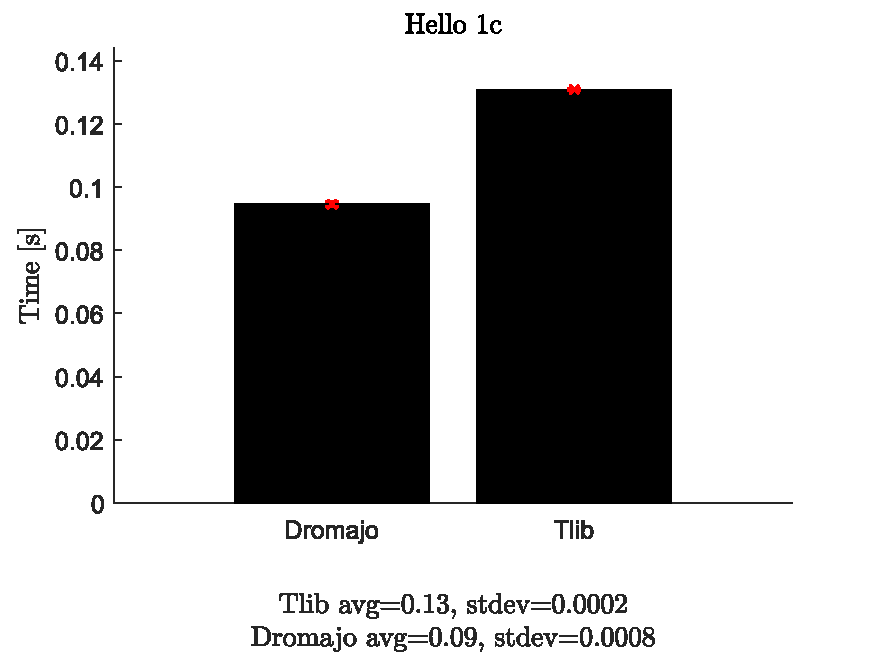
\includegraphics[width=0.6\textwidth]{figures/benchmarks/Hello1c.pdf}
	\caption{Zephyr RTOS boot times}
\end{figure}
\noindent
\textbf{Qualitative evaluation}: Both simulators were able to correctly boot up Zephyr RTOS.
\vspace*{15px}

\subsection{Zephyr RTOS $\pi$ calculating sample}

\begin{figure}[h]
    \centering
    \begin{subfigure}{0.5\textwidth}
      \centering
      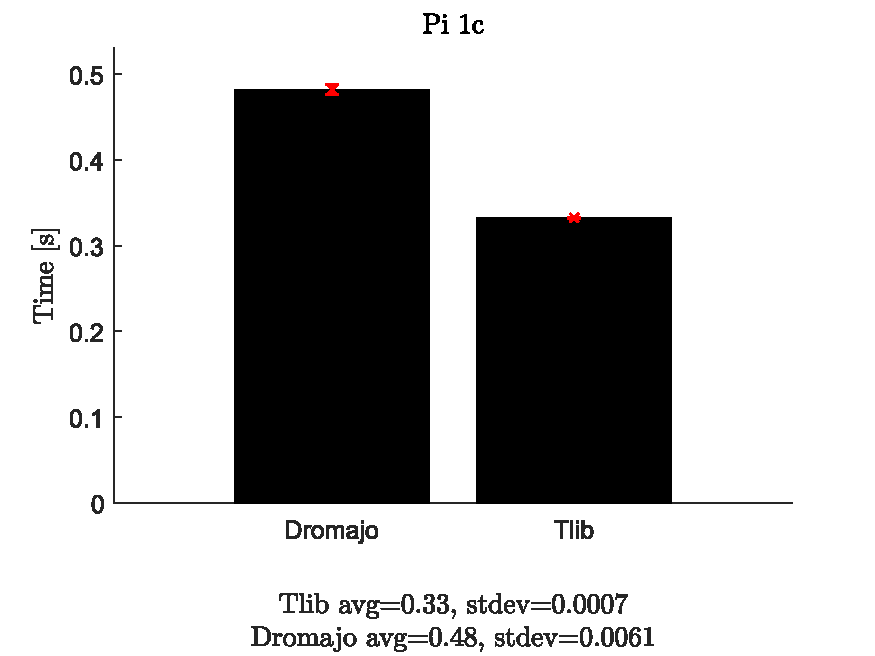
\includegraphics[width=1.2\linewidth]{figures/benchmarks/Pi1c.pdf}
    \end{subfigure}%
    \begin{subfigure}{0.5\textwidth}
      \centering
      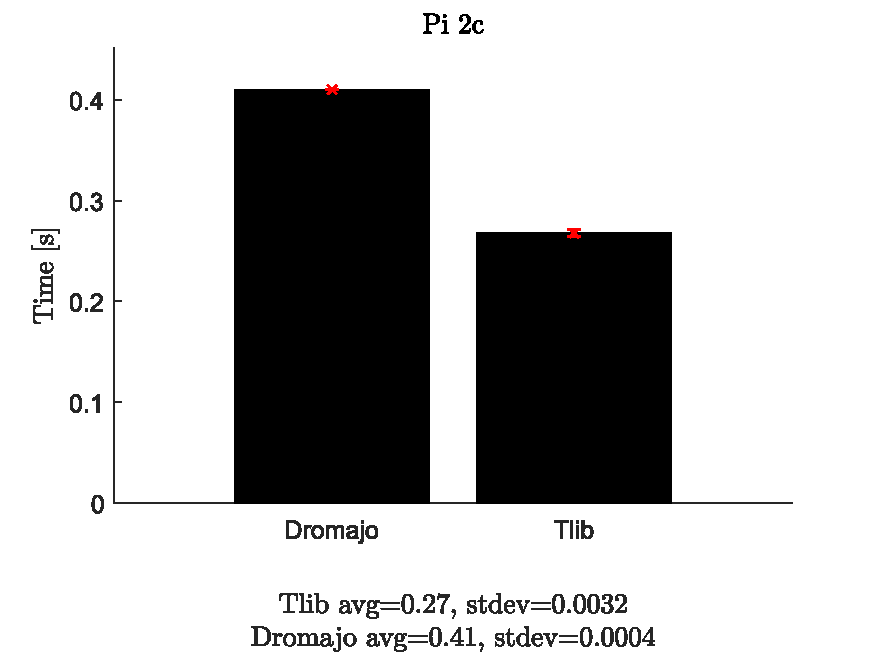
\includegraphics[width=1.2\linewidth]{figures/benchmarks/Pi2c.pdf}
    \end{subfigure}
    \caption{Zephyr RTOS $\pi$ calculating times}
\end{figure}
\textbf{Qualitative evaluation}: Both simulators have correctly executed the algorithm.
%Frankly speaking, I feel these will be much better if they had the samy Y scale... That applies to all 1c/2c graphs

\pagebreak

\subsection{Zephyr RTOS TensorFlow Lite Micro Module}

\begin{figure}[h]
    \centering
    \begin{subfigure}{0.5\textwidth}
      \centering
      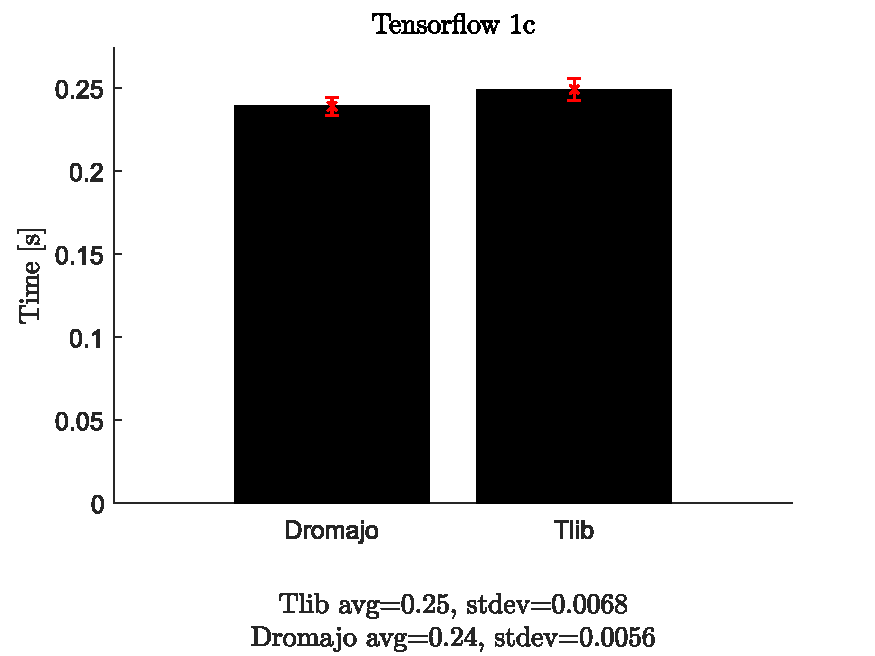
\includegraphics[width=1.2\linewidth]{figures/benchmarks/Tensorflow1c.pdf}
    \end{subfigure}%
    \begin{subfigure}{0.5\textwidth}
      \centering
      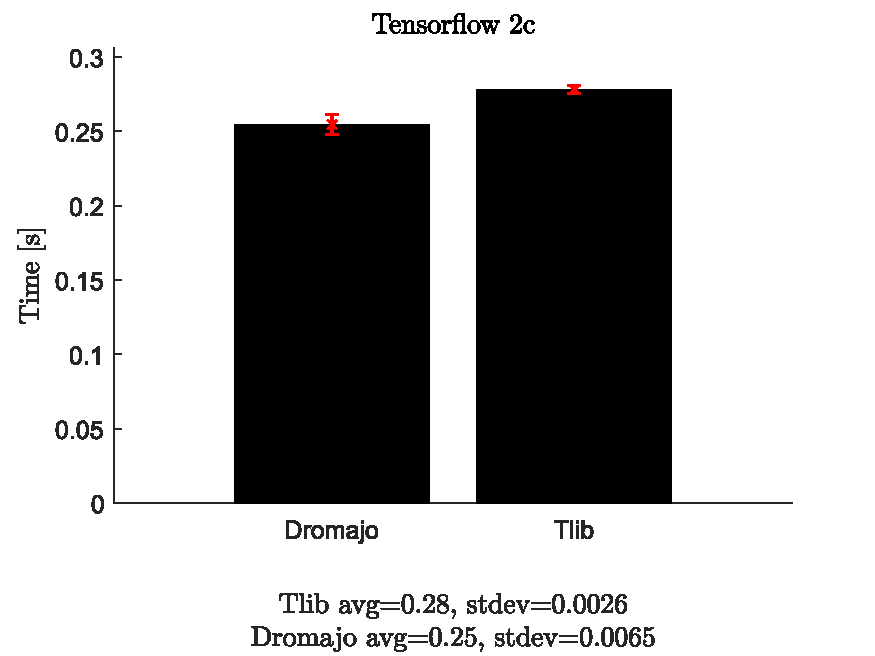
\includegraphics[width=1.2\linewidth]{figures/benchmarks/Tensorflow2c.pdf}
    \end{subfigure}
    \caption{Zephyr RTOS Tensorflow execution time}
\end{figure}
\textbf{Qualitative evaluation}: Both simulators have correctly executed the algorithm.
\vspace*{15px}

\subsection{Linux kernel boot-up}

\begin{figure}[h]
    \centering
    \begin{subfigure}{0.5\textwidth}
      \centering
      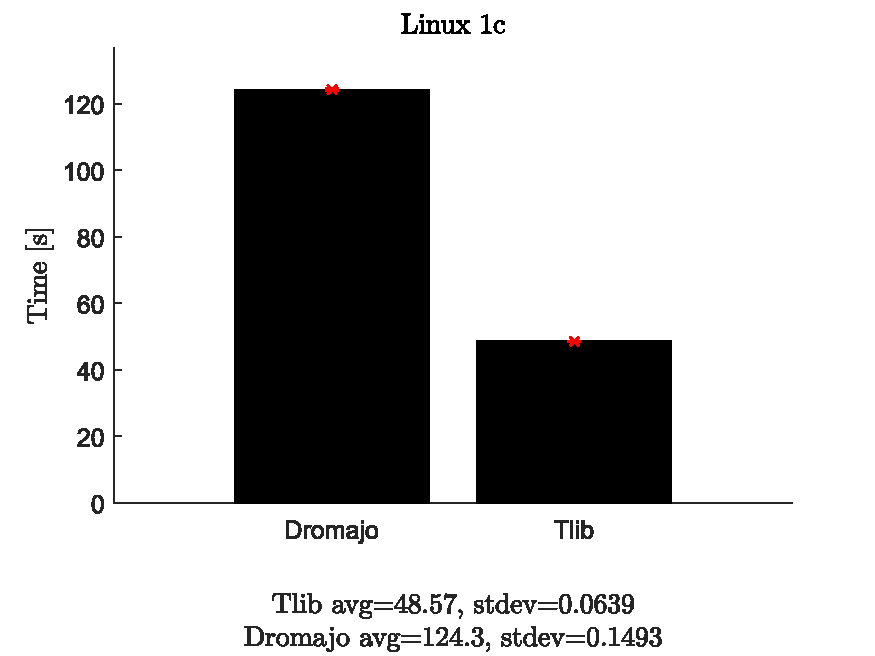
\includegraphics[width=1.2\linewidth]{figures/benchmarks/Linux1c.pdf}
    \end{subfigure}%
    \begin{subfigure}{0.5\textwidth}
      \centering
      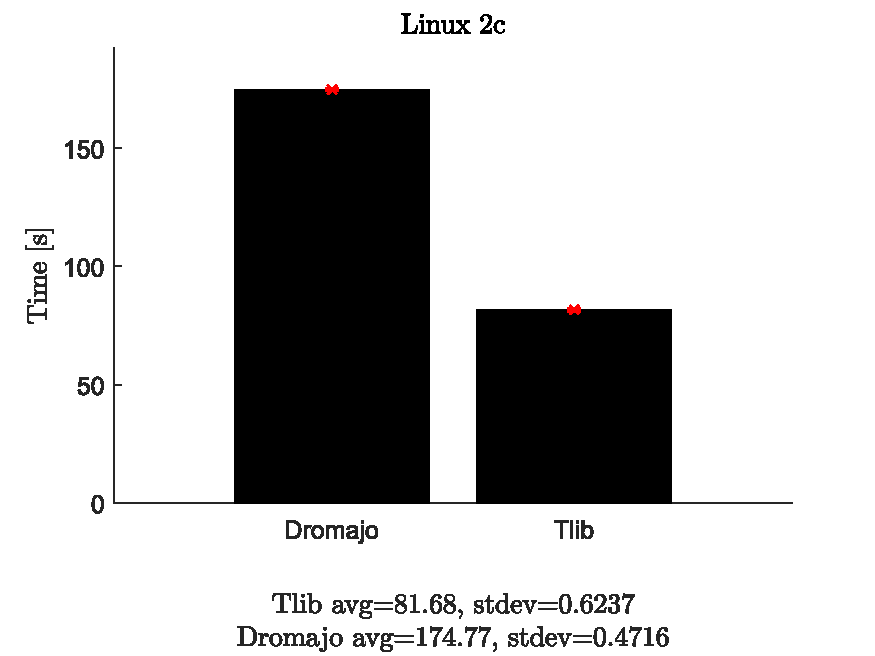
\includegraphics[width=1.2\linewidth]{figures/benchmarks/Linux2c.pdf}
    \end{subfigure}
    \caption{Zephyr RTOS Tensorflow execution time}
\end{figure}
\textbf{Qualitative evaluation}: Both simulators have correctly brought up the Linux kernel.
\vspace*{15px}

\noindent
The Linux kernel, being the biggest benchmark performed, generates a lot of logs on the UART console. This opened up a
possiblity to use Renode Log Tester to trace the time between each new message. This approach is called
\textit{Profiling} and is most typically used to perform a performance analysis for code execution. While some events
might be ommited (non-log emitting events), it is still an interesting data source that is worth investigating.

\pagebreak

\subsection{Linux boot profiling}
This section will provide two types of charts:
\begin{itemize}
    \item{\textbf{Boot profile chart}, a graph on a plane of virtual time versus host time. Each point represents a
    UART console message at a given point in time. This plot represents two pieces of information, the cumulative
    speedup or slowdown and the rate of change of the beforementioned characteristic. The increasing slope means that
    simulating the virtual processor, at this point, takes more time than is passing in real time. The decreasing slope
    represents the case when the simulated CPU is executing instructions faster than real time. If the chart slope
    matches the gray line slope, the simulated processor is executing instructions at exactly realtime speed.
    The gray line represents the "one-to-one" time mapping. If the execution chart is above this line, this means
    that the virtual CPU is lagging behind the real time and vice versa.}
    %
    \item{\textbf{Cumulative speedup chart}, provides a normalised version of the boot profile chart.
    The gray y-axis line represents "one-to-one" time mapping, with the same interpretation as in the boot profile
    chart.}
\end{itemize}

\pagebreak

%This graph is not readable! Really, even on serious zoom. I suggest rotating it clockwise 90 deg and increasing fonts
% also what is ioaccesses? I would also add the "prompt" event
\subsection*{Linux boot profiling - Tlib}
\begin{figure}[h]
	\centering
    \hspace*{-2cm}
	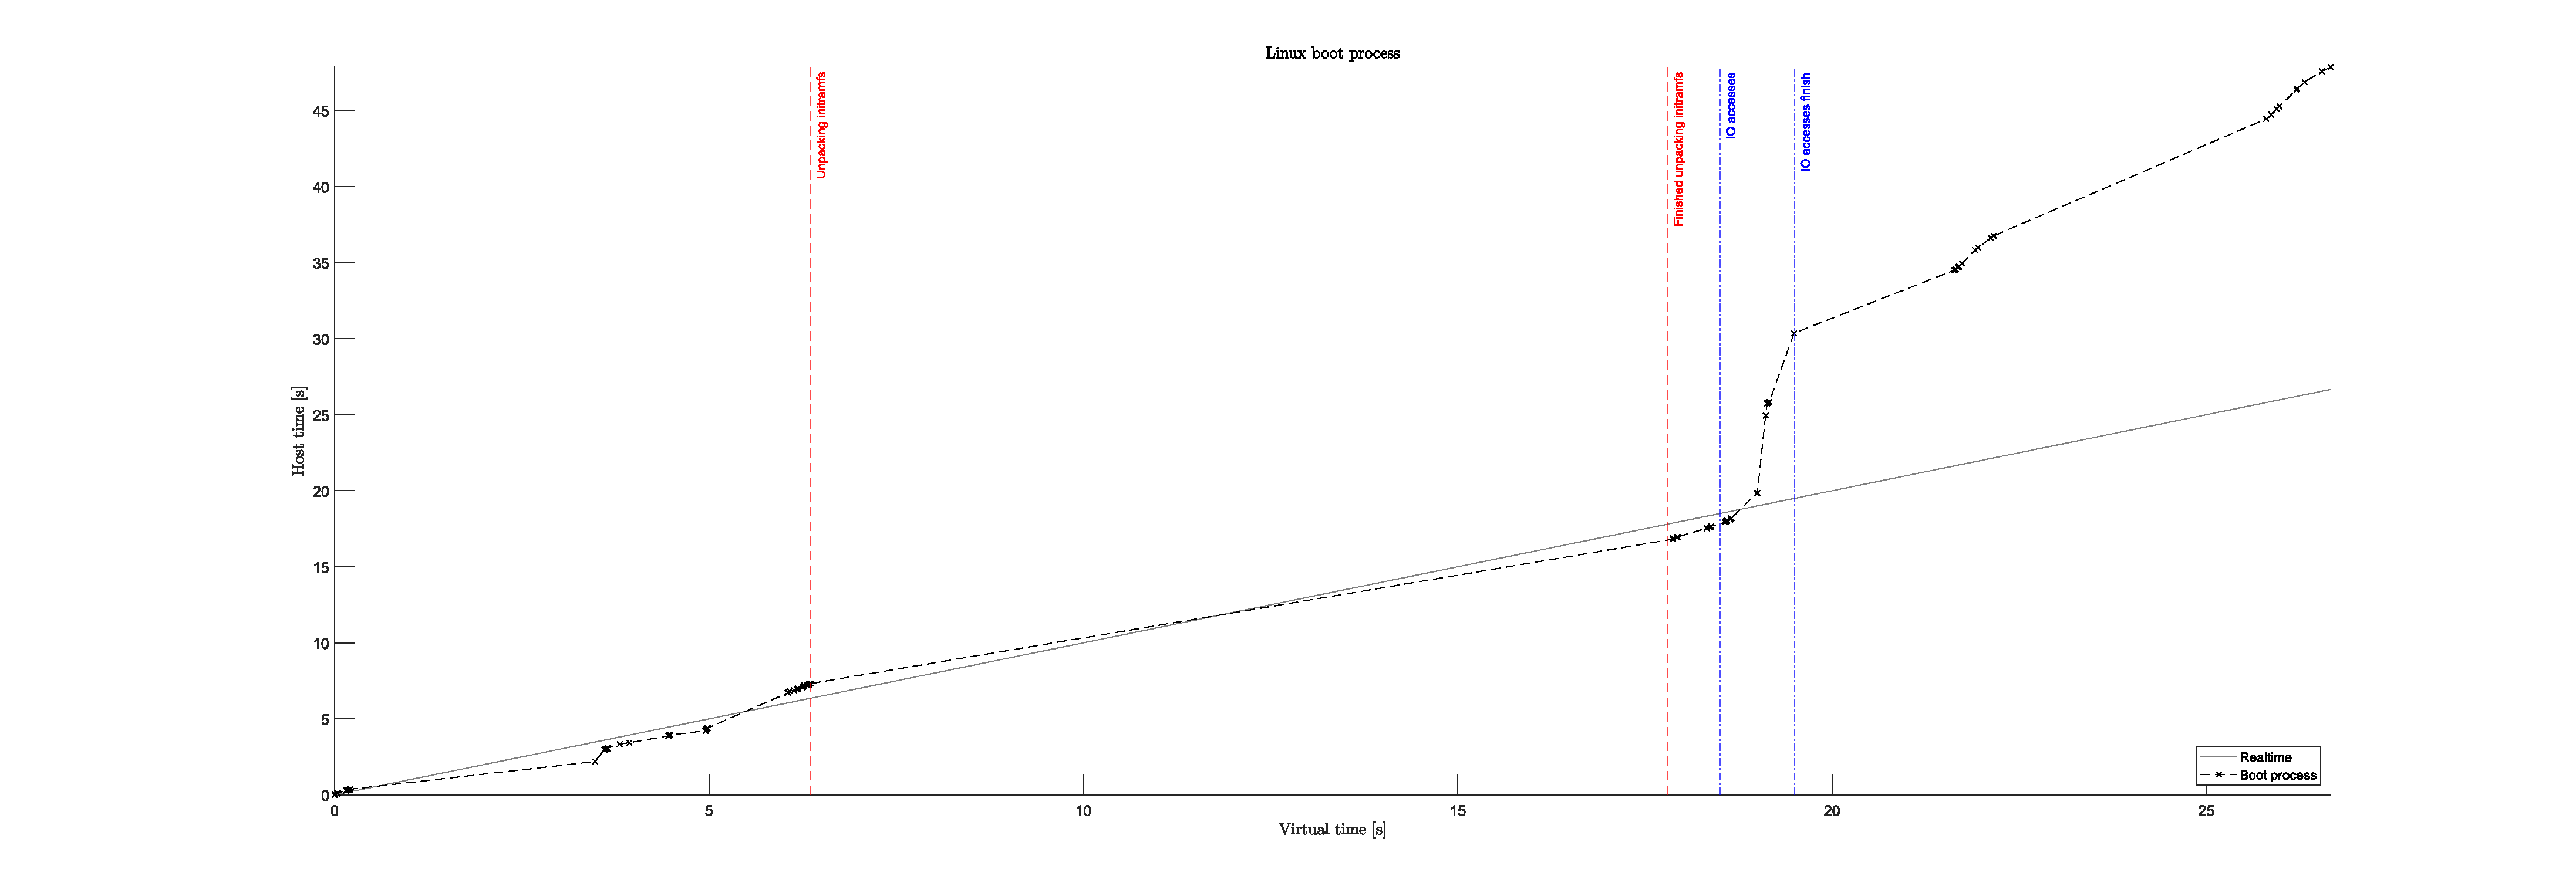
\includegraphics[width=1.2\textwidth]{figures/benchmarks/linux_boot/adnotated/TlibBoot.pdf}
	\caption{Linux boot profile chart - Translation Libraries}
\end{figure}

\noindent
The translation-based CPU was able to maintain a one-to-one virtual host time relation for most of
its execution, only falling behind when the I/O devices were heavily accessed. This is expected, as this mode of memory
access is not a subject to optimization methods described in the Chapter 3. Additionally, these accesses require a C
$\rightarrow$ C\# callback, which is also noticeably slow. After these accesses have been completed, the slope of the
chart returns to almost realtime, but not quite reaching it.

The area bounded by the red markers represents the time when the Linux kernel payload was unpacking initramfs. In terms
of the Linux kernel, this means extracting the initialization utilities from the \textit{gzip} archive into the
device random access memory, allowing the kernel to use RAM as a temporary rootfs. Since the boot process is not
progressing any further, it is not sending any messages to the UART device, thus expalining the lack of the data
points.

% same as above
\begin{figure}[h]
	\centering
    \hspace*{-2cm}
	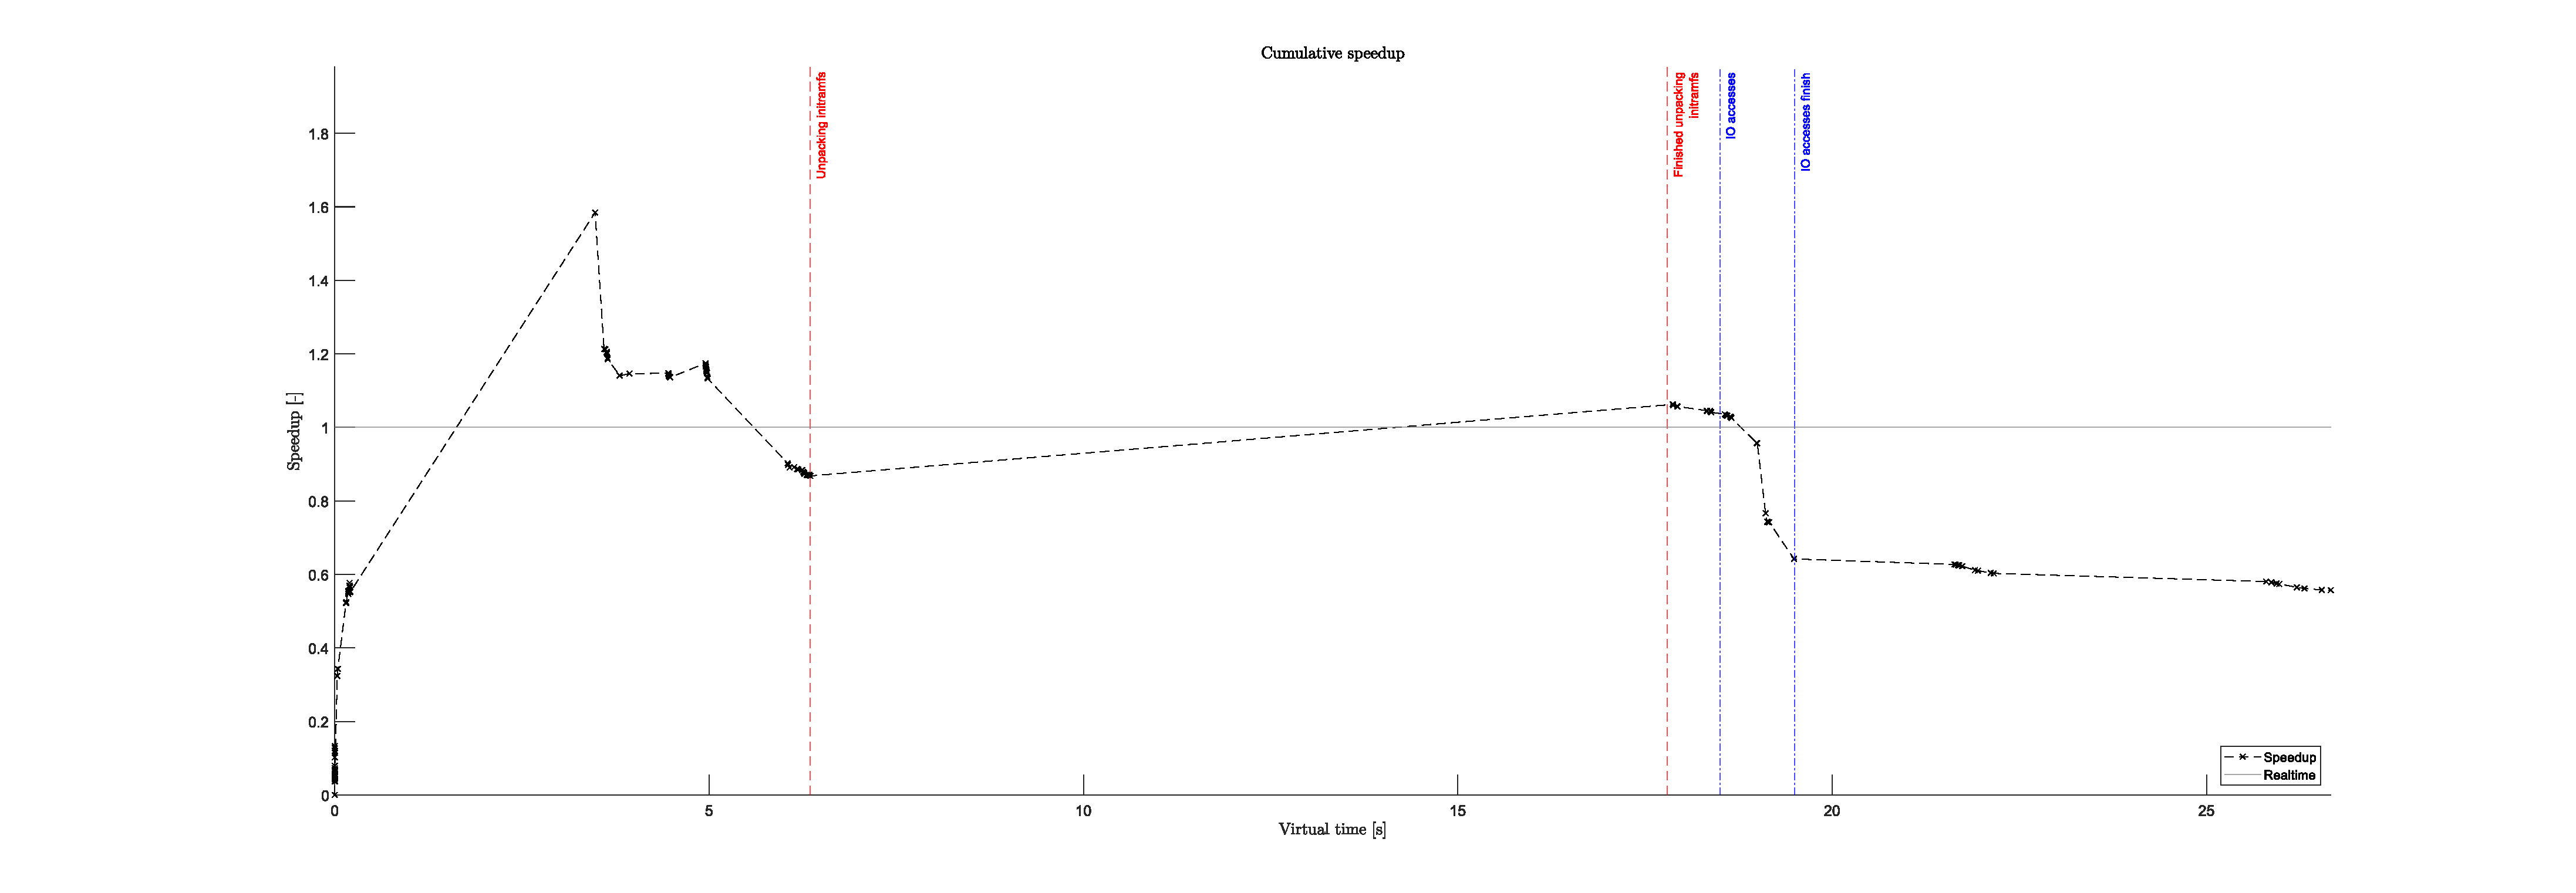
\includegraphics[width=1.2\textwidth]{figures/benchmarks/linux_boot/adnotated/TlibSpeedup.pdf}
	\caption{Linux speedup chart - Translation Libraries}
\end{figure}

\pagebreak

\subsection*{Linux boot profiling - Dromajo}

\begin{figure}[h]
	\centering
    \hspace*{-2cm}
	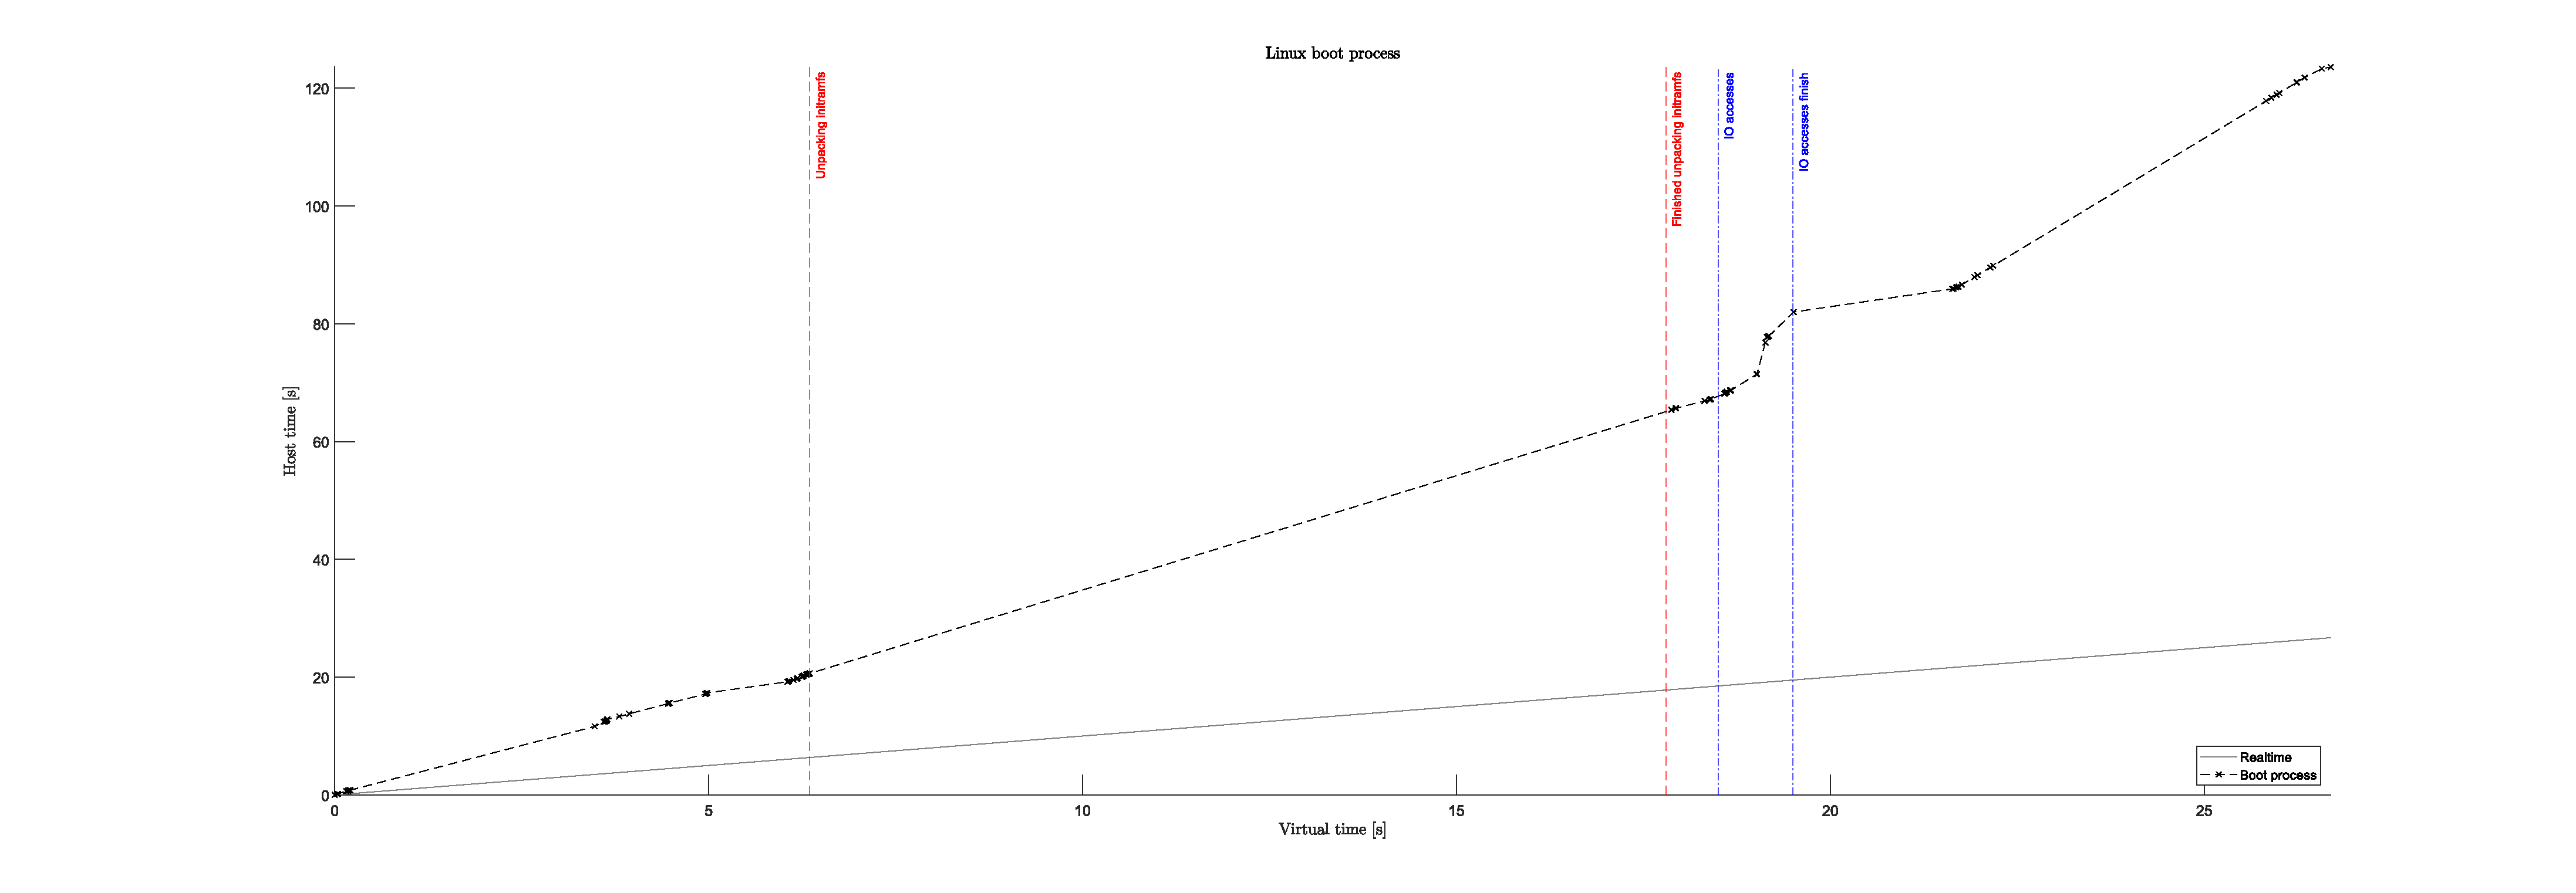
\includegraphics[width=1.2\textwidth]{figures/benchmarks/linux_boot/adnotated/DromajoBoot.pdf}
	\caption{Linux boot profile chart - Dromajo}
\end{figure}

\noindent
The Dromajo simulated CPU was not able to maintain a one-to-one virtual host time relation, it has immediately fallen
behind the real time execution. The characteristics of the chart are the same as in the Translation Libraries case, but the
%but the speedup graph is always much lower than one?
execution slope is always much bigger than one.

\begin{figure}[h]
	\centering
    \hspace*{-2cm}
	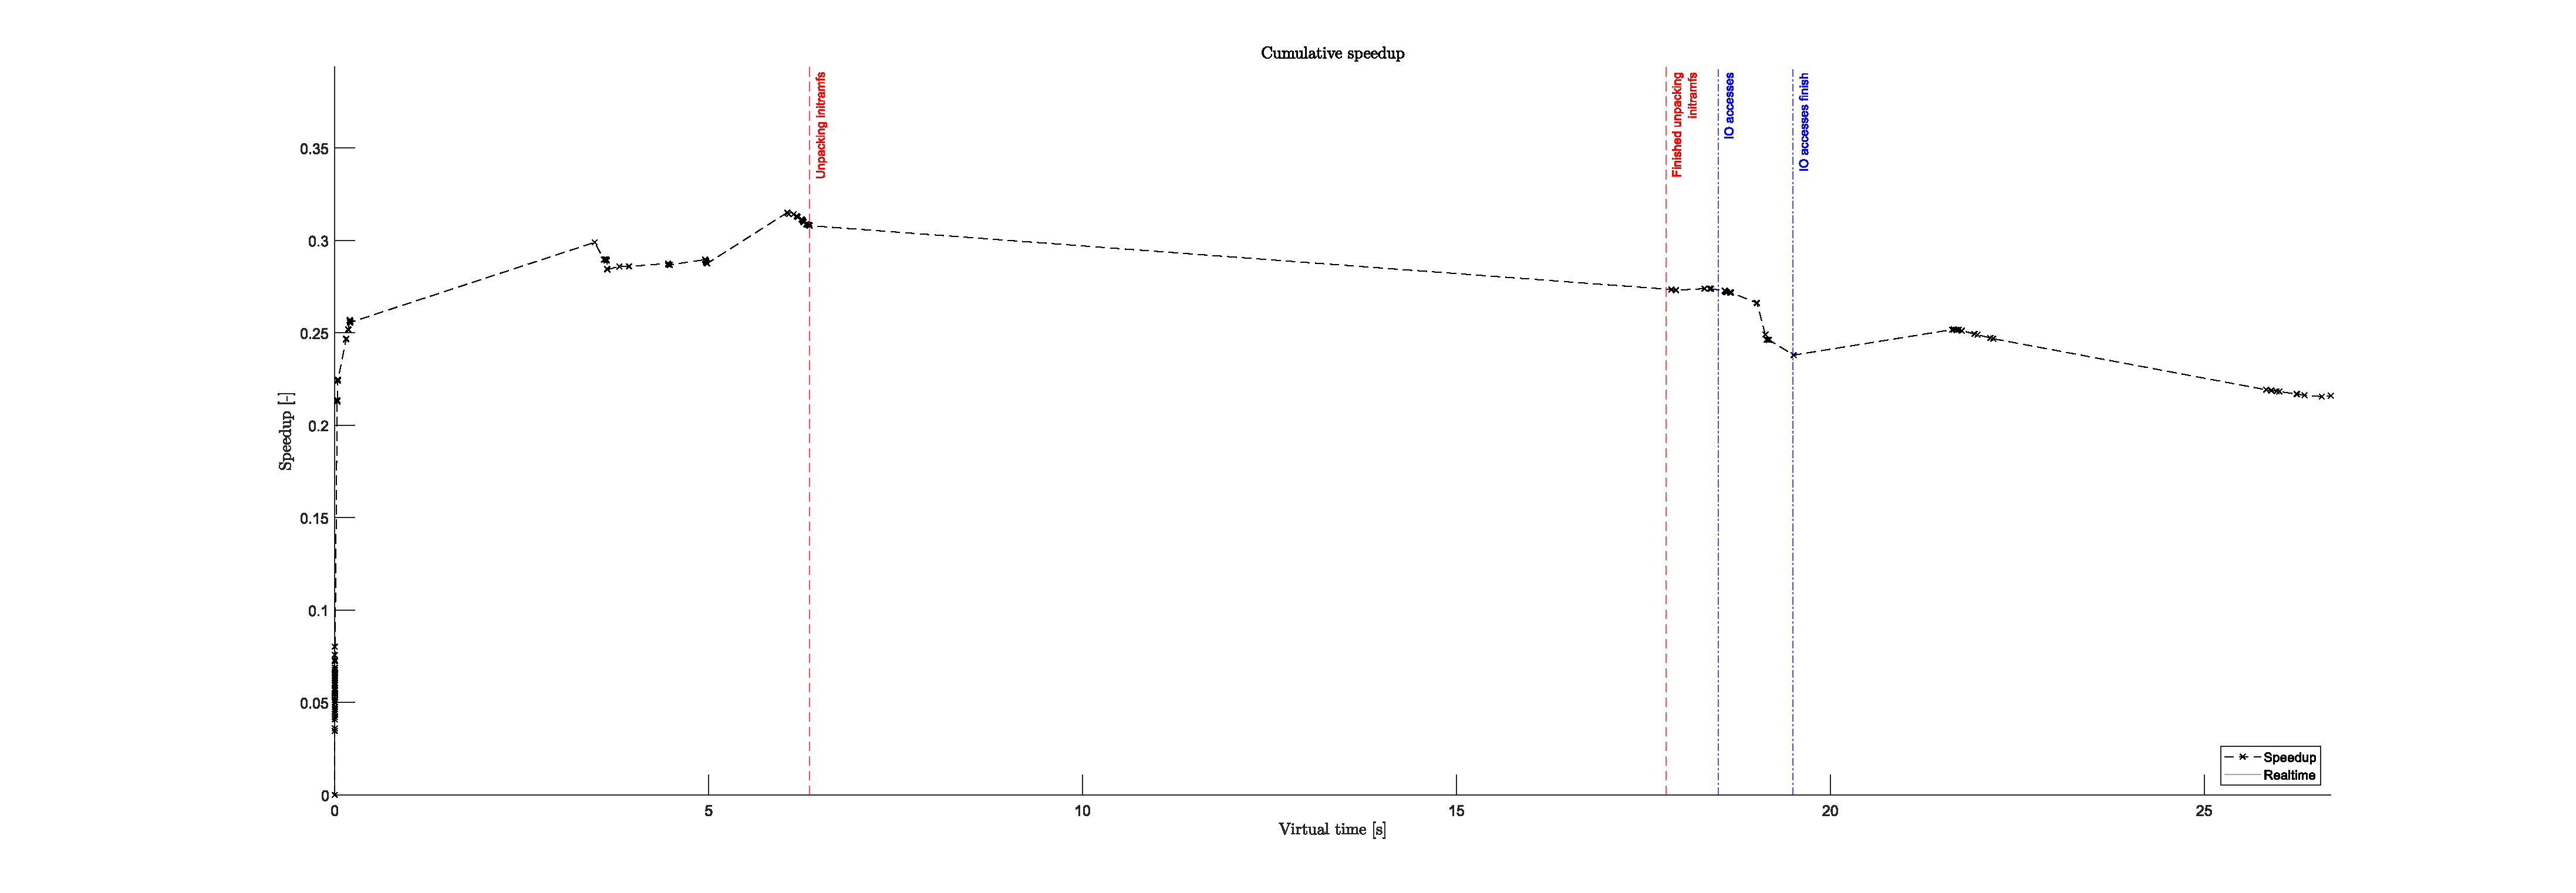
\includegraphics[width=1.2\textwidth]{figures/benchmarks/linux_boot/adnotated/DromajoSpeedup.pdf}
	\caption{Linux speedup chart - Dromajo}
\end{figure}

\pagebreak

\section{Performance conclusions}

\begin{table}[h]
    \centering
    \begin{tabular}{l|l|l}
    Benchmark             & Translation Libraries & Dromajo  \\ \hline
    Zephyr boot-up        & 0.13                  & 0.09     \\ \hline
    Zephyr $\pi$ calculation & 0.33               & 0.48     \\ \hline
    Zephyr Tensorflow     & 0.25                  & 0.24     \\ \hline
    Linux kernel boot-up  & 45.57                 & 124.3
    \end{tabular}
    \caption{Benchmark summary results for single core tests}
\end{table}

\begin{table}[h]
    \centering
    \begin{tabular}{l|l|l}
    Benchmark             & Translation Libraries & Dromajo  \\ \hline
    Zephyr boot-up        & -                     & -        \\ \hline
    Zephyr $\pi$ calculation & 0.27               & 0.41     \\ \hline
    Zephyr Tensorflow     & 0.28                  & 0.25     \\ \hline
    Linux kernel boot-up  & 81.68                 & 174.77
    \end{tabular}
    \caption{Benchmark summary results for dual core tests}
\end{table}

\noindent
Both of the simulation methods managed to pass the qualitative evaluation. The virtual CPUs behaved in a stable
and expected way. A low standard deviation in both cases also confirms the stability and repeatability of the test
results.
%Standard deviation for 3 runs is... questionable. If someone asks you about it, you might be in trouble. Just saying.

In terms of performance, the Translation Libraries simulated central processing unit performs better at every more
complex test, by as much as two times in the Linux test. This behavior is a merit of the block caching and chaining,
exceptionally speeding up the simulation process. The techniques applied in this method of simulation allow the virtual
processor to reach near real time execution performance.

The Dromajo simulated CPU performed better in the simpler payloads, such as booting the Zephyr RTOS, where the
optimization techniques used in the translation approach had become a noticeably big overhead - the process of
% This sentence is rewritable ;-)
block caching and chaining had significant cost and did not have any noticeable effect on the simulation, as it had
already ended. This suggests that for small payloads block caching and chaining is simply not a worthwile optimization
method.


\chapter{Summary and conclusions}

\section{Summary}

The thesis offers a comprehensive examination of various simulation methods employed in the field, ranging from
relatively simple API emulators to complex whole-system simulators. It delves into the fundamental limitations
encountered in the design of simulators, challenges faced by users and developers, and the crucial need for such
software in the context of automatic control, robotics, Internet of Things (IoT), and edge computing solutions.
Additionally, the thesis provides an overview of types of mechanisms utilized in central processing unit emulation
software and their intended purposes

The thesis specifically focuses on two fundamental approaches used in CPU simulators: the translation approach and the
interpretation approach. The translation approach is examined in-depth, with the analysis of mechanisms of code
translation using TCG back-end and front-end, providing a sample of translated code, and examination of the execution flow
in such simulators. Special attention is given to the optimization methods employed in these simulators, such as
translation block caching and chaining. This analysis concludes with an examination of the code flow, exception and
interrupt handling, and the important concept of helper functions. This approach is described using the example of QEMU
and Renode Translation Libraries, with accompanying code samples.

The interpretation approach is also extensively examined, with the work delving into the methods employed in such
simulators, providing an in-depth examination of the inner workings of the Dromajo simulator, and comparing the two
simulation techniques. The author goes on to implement the interpretation processor simulator (Dromajo) with Renode.
The work describes the necessary interfaces for CPU emulation, explains
the process of integrating an API into an existing C library, and details the steps involved in the integration of a new
processor emulator with the Renode framework. Finally, the thesis presents a performance analysis of both types of
simulators and conducts a comparison of the results.

\pagebreak

\section{Conclusions}

The performance analysis conducted in this work concludes that translation processor emulators exhibit a substantial
performance advantage in terms of execution speed. This conclusion holds true for the majority of payloads, with the
exception of less complex binaries, where the optimization methods employed in the translation approach can create a
non-negligible overhead.

However, this advantage in execution speed comes at the cost of increased memory usage and much higher complexity in
the codebase. These trade-offs must be carefully considered when choosing between translation and interpretation
simulators, as they might not only have an instantaneous impact on the performance of the project but might also
have long-lasting negative effects in terms of the complicated codebase, lower maintainability and reduced
expandability.
% this is quite negative, I must say...

Interpretation simulators usually also offer the additional advantage of being fully portable, they do not need
to be heavily customized to run on another platform. This is not the case with translation simulators, which must
implement an additional \textit{intermediate representation} to host the translation layer, and they need to maintain architecture-specific backends.

\section{Future work}

There are several areas where future work can be done to further improve the simulation methods discussed in this
thesis. Some possible directions for future research include:

\begin{itemize}
    \item{\textbf{Developing more advanced interpretation simulators}: The interpretation approach has the advantage of
     being fully portable, but it also has a lower performance compared to translation simulators. Research can be done
     to develop more optimization methods, that can improve performance while still maintaining the advantages of
     portability and ease of maintainability and expansion.}
     %
     \item{\textbf{Improving the portability of translation simulators}: Despite great performance, translation
     simulators suffer in terms of portability. Further work can be done to explore new approaches to this method, in
     order to improve the ease of maintainability, expandability, and overall developer friendliness.}
     %
     \item{\textbf{Real time simulation}: Many simulation applications require real-time performance, like control
     systems, robotics, and other dynamic systems. Further research can be done to explore new methods for achieving
     real-time performance in simulation, such as using multi-core processors, distributed computing, or specialized
     hardware.}
     %
     \item{\textbf{Further evaluation}: Additional tests can be performed against the given solutions to further increase understanding of their strengths and shortcomings.
     More detailed analysis of impact of specific optimisations of the translation-based simulator can also be performed, to gauge their relative benefit against maintenance cost.}
\end{itemize}


%--------------------------------------
% Literatura
%--------------------------------------

\bibliographystyle{unsrt}{\raggedright\sloppy\small\bibliography{bibliografia}}

%--------------------------------------
% Dodatki
%--------------------------------------

\cleardoublepage\appendix%
\newpage
% Removing all includes from this section breaks some conditional
\if

\begin{appendices}
   \chapter{Definitions}

\end{appendices}

%--------------------------------------
% Informacja o prawach autorskich
%--------------------------------------

\ppcolophon

\end{document}
